\begin{comment}

\begin{table}
\centering 
\begin{tabular}
{lcrclcrcl@{\hspace{0.1cm}}cc}

\multicolumn{11}{c}{Precision (strict)}\\
\hline
Task && \multicolumn{3}{c}{ILP}  && \multicolumn{3}{c}{PAUM} && \\
\hline
start             && 0.946 & $\pm$ & 0.09 && 0.668 & $\pm$ & 0.18 & $\bullet$\\
damage            && 0.916 & $\pm$ & 0.16 && 0.864 & $\pm$ & 0.21 &          \\
end\_subtree      && 0.687 & $\pm$ & 0.34 && 0.552 & $\pm$ & 0.24 & $\bullet$\\
injuries          && 0.663 & $\pm$ & 0.36 && 0.417 & $\pm$ & 0.29 & $\bullet$\\
fatalities        && 0.940 & $\pm$ & 0.24 && 0.347 & $\pm$ & 0.40 & $\bullet$\\
profesional\_unit && 0.716 & $\pm$ & 0.19 && 0.678 & $\pm$ & 0.15 &          \\
amateur\_unit     && 0.841 & $\pm$ & 0.28 && 0.561 & $\pm$ & 0.30 & $\bullet$\\
\hline
overall           && 0.816 & $\pm$ & 0.28 && 0.584 & $\pm$ & 0.31 & $\bullet$\\
\hline
\\


\multicolumn{11}{c}{Recall (strict)}\\
\hline
Task && \multicolumn{3}{c}{ILP}  && \multicolumn{3}{c}{PAUM} && \\
\hline
start             && 0.906 & $\pm$ & 0.15 && 0.978 & $\pm$ & 0.07 & $\circ$\\
damage            && 0.827 & $\pm$ & 0.26 && 0.905 & $\pm$ & 0.23 &        \\
end\_subtree      && 0.237 & $\pm$ & 0.24 && 0.632 & $\pm$ & 0.26 & $\circ$\\
injuries          && 0.531 & $\pm$ & 0.36 && 0.797 & $\pm$ & 0.25 & $\circ$\\
fatalities        && 0.440 & $\pm$ & 0.48 && 0.653 & $\pm$ & 0.45 & $\circ$\\
profesional\_unit && 0.615 & $\pm$ & 0.16 && 0.813 & $\pm$ & 0.17 & $\circ$\\
amateur\_unit     && 0.850 & $\pm$ & 0.27 && 0.954 & $\pm$ & 0.10 & $\circ$\\
\hline
overall           && 0.629 & $\pm$ & 0.37 && 0.819 & $\pm$ & 0.28 & $\circ$\\
\hline
\\

\multicolumn{11}{c}{$F_1$ measure (strict)}\\
\hline
Task && \multicolumn{3}{c}{ILP}  && \multicolumn{3}{c}{PAUM} && \\
\hline
start             && 0.916 & $\pm$ & 0.10 && 0.779 & $\pm$ & 0.13 & $\bullet$\\
damage            && 0.833 & $\pm$ & 0.22 && 0.845 & $\pm$ & 0.23 &          \\
end\_subtree      && 0.277 & $\pm$ & 0.25 && 0.562 & $\pm$ & 0.21 & $\circ$\\
injuries          && 0.512 & $\pm$ & 0.35 && 0.488 & $\pm$ & 0.25 &          \\
fatalities        && 0.437 & $\pm$ & 0.48 && 0.300 & $\pm$ & 0.37 &          \\
profesional\_unit && 0.651 & $\pm$ & 0.15 && 0.729 & $\pm$ & 0.14 & $\circ$\\
amateur\_unit     && 0.770 & $\pm$ & 0.32 && 0.646 & $\pm$ & 0.30 & $\bullet$\\
\hline
overall           && 0.628 & $\pm$ & 0.36 && 0.621 & $\pm$ & 0.30 &  \\
\hline
\multicolumn{11}{c}{$\circ$, $\bullet$ statistically significant improvement or degradation}\\
\end{tabular}

\caption{Evaluation on Czech Fireman dataset} \label{tab:ch60_fir_eval}
\end{table}



\begin{table}
\centering 
\begin{tabular}
{lcrclcrcl@{\hspace{0.1cm}}cc}

\multicolumn{11}{c}{Training time (in seconds)}\\
\hline
Task && \multicolumn{3}{c}{ILP}  && \multicolumn{3}{c}{PAUM} && \\
\hline
start              &  & 280.7 &  $\pm$  & 21.5 &  & 24.01 &  $\pm$  & 2.08 &  $\circ$\\
damage             &  & 236.2 &  $\pm$  & 16.2 &  & 24.79 &  $\pm$  & 2.42 &  $\circ$\\
end\_subtree       &  & 971.4 &  $\pm$  & 77.8 &  & 24.90 &  $\pm$  & 2.33 &  $\circ$\\
injuries           &  & 938.1 &  $\pm$  & 34.8 &  & 24.77 &  $\pm$  & 2.20 &  $\circ$\\
fatalities         &  & 477.0 &  $\pm$  & 64.4 &  & 24.64 &  $\pm$  & 2.12 &  $\circ$\\
profesional\_unit  &  & 1615.6 &  $\pm$ & 84.9 &  & 24.51 &  $\pm$  & 2.04 &  $\circ$\\
amateur\_unit      &  & 259.3 &  $\pm$  & 15.5 &  & 26.07 &  $\pm$  & 2.60 &  $\circ$\\
\hline
overall            &  & 682.6 &  $\pm$  & 481.9 & & 24.81 &  $\pm$  & 2.32 &  $\circ$\\
\hline
\\

\multicolumn{11}{c}{Training time (in seconds)}\\
\hline
Task && \multicolumn{3}{c}{ILP}  && \multicolumn{3}{c}{PAUM} && \\
\hline
start              &  & 7.211 &  $\pm$  & 0.10 &  & 2.095 &  $\pm$  & 0.08 &  $\circ$\\
damage             &  & 7.295 &  $\pm$  & 0.14 &  & 2.241 &  $\pm$  & 0.10 &  $\circ$\\
end\_subtree       &  & 7.275 &  $\pm$  & 0.11 &  & 2.339 &  $\pm$  & 0.05 &  $\circ$\\
injuries           &  & 7.278 &  $\pm$  & 0.09 &  & 2.200 &  $\pm$  & 0.08 &  $\circ$\\
fatalities         &  & 7.149 &  $\pm$  & 0.07 &  & 2.268 &  $\pm$  & 0.11 &  $\circ$\\
profesional\_unit  &  & 7.193 &  $\pm$  & 0.10 &  & 2.297 &  $\pm$  & 0.01 &  $\circ$\\
amateur\_unit      &  & 7.218 &  $\pm$  & 0.15 &  & 2.275 &  $\pm$  & 0.04 &  $\circ$\\
\hline
overall            &  & 7.231 &  $\pm$  & 0.12 &  & 2.245 &  $\pm$  & 0.10 &  $\circ$\\
\hline

\multicolumn{11}{c}{$\circ$ statistically significant increase (not improvement in this case)}\\
\end{tabular}

\medskip
The time in this table is cumulative (sum over all folds in one experiment run).

\caption{Time spent by ML engines on the Czech Fireman dataset.} \label{tab:ch60_fir_time}
\end{table}







\clearpage
aaa

\vspace{1.1cm}


\begin{longtable}{|r|r|l||rcl|rcl|c|}
\hline
\multirow{2}{*}{task} & \multicolumn{2}{|c||}{\multirow{2}{*}{measured quantity}} & \multicolumn{3}{|c|}{ILP} & \multicolumn{3}{|c|}{PAUM} & \multirow{2}{*}{ stat. sig.}\\
\cline{4-9}
  & \multicolumn{2}{|c||}{} &  avg  &    &  stdev  &  avg  &    &  stdev  & \\
\hline
\endhead
\hline
\hline
\multirow{11}{*}{\begin{sideways}start\end{sideways} } & \multirow{4}{*}{Number} &  Correct  & 3.780 &  $\pm$  & 0.95 & 4.100 &  $\pm$  & 0.91 &  $\circ$\\
\cline{3-10}
 &  &  Missing  & 0.420 &  $\pm$  & 0.64 & 0.100 &  $\pm$  & 0.30 &  $\bullet$\\
\cline{3-10}
 &  &  Spurious  & 0.300 &  $\pm$  & 0.54 & 2.500 &  $\pm$  & 1.82 &  $\circ$\\
\cline{3-10}
 &  &  Overlap  & 0.000 &  $\pm$  & 0.00 & 0.000 &  $\pm$  & 0.00 &   \\
\cline{2-10}
 & \multirow{3}{*}{Strict} &  Prec.  & 0.946 &  $\pm$  & 0.09 & 0.668 &  $\pm$  & 0.18 &  $\bullet$\\
\cline{3-10}
 &  &  Rec.  & 0.906 &  $\pm$  & 0.15 & 0.978 &  $\pm$  & 0.07 &  $\circ$\\
\cline{3-10}
 &  &  $F_1$  & 0.916 &  $\pm$  & 0.10 & 0.779 &  $\pm$  & 0.13 &  $\bullet$\\
\cline{2-10}
 & Lenient &  $F_1$  & 0.916 &  $\pm$  & 0.10 & 0.779 &  $\pm$  & 0.13 &  $\bullet$\\
\cline{2-10}
 & Average &  $F_1$  & 0.916 &  $\pm$  & 0.10 & 0.779 &  $\pm$  & 0.13 &  $\bullet$\\
\cline{2-10}
 & \multirow{2}{*}{Time} &  training  & 280.668 &  $\pm$  & 21.47 & 24.011 &  $\pm$  & 2.08 &  $\bullet$\\
\cline{3-10}
 &  &  testing  & 7.211 &  $\pm$  & 0.10 & 2.095 &  $\pm$  & 0.08 &  $\bullet$\\
\hline
\hline
\multirow{11}{*}{\begin{sideways}damage\end{sideways} } & \multirow{4}{*}{Number} &  Correct  & 1.520 &  $\pm$  & 0.97 & 1.800 &  $\pm$  & 1.16 &  $\circ$\\
\cline{3-10}
  &  &  Missing  & 0.460 &  $\pm$  & 0.71 & 0.200 &  $\pm$  & 0.40 &  $\bullet$\\
\cline{3-10}
  &  &  Spurious  & 0.240 &  $\pm$  & 0.48 & 0.520 &  $\pm$  & 0.95 &  $\circ$\\
\cline{3-10}
  &  &  Overlap  & 0.020 &  $\pm$  & 0.14 & 0.000 &  $\pm$  & 0.00 &   \\
\cline{2-10}
  & \multirow{3}{*}{Strict} &  Prec.  & 0.916 &  $\pm$  & 0.16 & 0.864 &  $\pm$  & 0.21 &   \\
\cline{3-10}
  &  &  Rec.  & 0.827 &  $\pm$  & 0.26 & 0.905 &  $\pm$  & 0.23 &   \\
\cline{3-10}
  &  &  $F_1$  & 0.833 &  $\pm$  & 0.22 & 0.845 &  $\pm$  & 0.23 &   \\
\cline{2-10}
  & Lenient &  $F_1$  & 0.843 &  $\pm$  & 0.21 & 0.845 &  $\pm$  & 0.23 &   \\
\cline{2-10}
  & Average &  $F_1$  & 0.838 &  $\pm$  & 0.21 & 0.845 &  $\pm$  & 0.23 &   \\
\cline{2-10}
  & \multirow{2}{*}{Time} &  training  & 236.184 &  $\pm$  & 16.17 & 24.791 &  $\pm$  & 2.42 &  $\bullet$\\
\cline{3-10}
  &  &  testing  & 7.295 &  $\pm$  & 0.14 & 2.241 &  $\pm$  & 0.10 &  $\bullet$\\
\hline
\hline
\multirow{11}{*}{\begin{sideways}end\_subtree\end{sideways} } & \multirow{4}{*}{Number} &  Correct  & 0.920 &  $\pm$  & 0.85 & 2.640 &  $\pm$  & 1.41 &  $\circ$\\
\cline{3-10}
  &  &  Missing  & 3.040 &  $\pm$  & 1.63 & 1.200 &  $\pm$  & 0.90 &  $\bullet$\\
\cline{3-10}
  &  &  Spurious  & 0.680 &  $\pm$  & 0.94 & 2.000 &  $\pm$  & 1.58 &  $\circ$\\
\cline{3-10}
  &  &  Overlap  & 0.240 &  $\pm$  & 0.62 & 0.360 &  $\pm$  & 0.60 &   \\
\cline{2-10}
  & \multirow{3}{*}{Strict} &  Prec.  & 0.687 &  $\pm$  & 0.34 & 0.552 &  $\pm$  & 0.24 &  $\bullet$\\
\cline{3-10}
  &  &  Rec.  & 0.237 &  $\pm$  & 0.24 & 0.632 &  $\pm$  & 0.26 &  $\circ$\\
\cline{3-10}
  &  &  $F_1$  & 0.277 &  $\pm$  & 0.25 & 0.562 &  $\pm$  & 0.21 &  $\circ$\\
\cline{2-10}
  & Lenient &  $F_1$  & 0.344 &  $\pm$  & 0.27 & 0.635 &  $\pm$  & 0.18 &  $\circ$\\
\cline{2-10}
  & Average &  $F_1$  & 0.310 &  $\pm$  & 0.25 & 0.598 &  $\pm$  & 0.18 &  $\circ$\\
\cline{2-10}
  & \multirow{2}{*}{Time} &  training  & 971.414 &  $\pm$  & 77.82 & 24.903 &  $\pm$  & 2.33 &  $\bullet$\\
\cline{3-10}
  &  &  testing  & 7.275 &  $\pm$  & 0.11 & 2.339 &  $\pm$  & 0.05 &  $\bullet$\\
\hline
\hline
\multirow{11}{*}{\begin{sideways}injuries\end{sideways} } & \multirow{4}{*}{Number} &  Correct  & 1.480 &  $\pm$  & 1.30 & 2.400 &  $\pm$  & 1.64 &  $\circ$\\
\cline{3-10}
  &  &  Missing  & 1.820 &  $\pm$  & 1.72 & 0.900 &  $\pm$  & 1.13 &  $\bullet$\\
\cline{3-10}
  &  &  Spurious  & 1.740 &  $\pm$  & 3.59 & 4.380 &  $\pm$  & 3.40 &  $\circ$\\
\cline{3-10}
  &  &  Overlap  & 0.000 &  $\pm$  & 0.00 & 0.000 &  $\pm$  & 0.00 &   \\
\cline{2-10}
  & \multirow{3}{*}{Strict} &  Prec.  & 0.663 &  $\pm$  & 0.36 & 0.417 &  $\pm$  & 0.29 &  $\bullet$\\
\cline{3-10}
  &  &  Rec.  & 0.531 &  $\pm$  & 0.36 & 0.797 &  $\pm$  & 0.25 &  $\circ$\\
\cline{3-10}
  &  &  $F_1$  & 0.512 &  $\pm$  & 0.35 & 0.488 &  $\pm$  & 0.25 &   \\
\cline{2-10}
  & Lenient &  $F_1$  & 0.512 &  $\pm$  & 0.35 & 0.488 &  $\pm$  & 0.25 &   \\
\cline{2-10}
  & Average &  $F_1$  & 0.512 &  $\pm$  & 0.35 & 0.488 &  $\pm$  & 0.25 &   \\
\cline{2-10}
  & \multirow{2}{*}{Time} &  training  & 938.101 &  $\pm$  & 34.76 & 24.770 &  $\pm$  & 2.20 &  $\bullet$\\
\cline{3-10}
  &  &  testing  & 7.278 &  $\pm$  & 0.09 & 2.200 &  $\pm$  & 0.08 &  $\bullet$\\
\hline
\hline
\multirow{11}{*}{\begin{sideways}fatalities\end{sideways} } & \multirow{4}{*}{Number} &  Correct  & 0.140 &  $\pm$  & 0.35 & 0.440 &  $\pm$  & 0.67 &  $\circ$\\
\cline{3-10}
  &  &  Missing  & 0.960 &  $\pm$  & 1.03 & 0.660 &  $\pm$  & 0.96 &  $\bullet$\\
\cline{3-10}
  &  &  Spurious  & 0.060 &  $\pm$  & 0.24 & 1.480 &  $\pm$  & 1.34 &  $\circ$\\
\cline{3-10}
  &  &  Overlap  & 0.000 &  $\pm$  & 0.00 & 0.000 &  $\pm$  & 0.00 &   \\
\cline{2-10}
  & \multirow{3}{*}{Strict} &  Prec.  & 0.940 &  $\pm$  & 0.24 & 0.347 &  $\pm$  & 0.40 &  $\bullet$\\
\cline{3-10}
  &  &  Rec.  & 0.440 &  $\pm$  & 0.48 & 0.653 &  $\pm$  & 0.45 &  $\circ$\\
\cline{3-10}
  &  &  $F_1$  & 0.437 &  $\pm$  & 0.48 & 0.300 &  $\pm$  & 0.37 &   \\
\cline{2-10}
  & Lenient &  $F_1$  & 0.437 &  $\pm$  & 0.48 & 0.300 &  $\pm$  & 0.37 &   \\
\cline{2-10}
  & Average &  $F_1$  & 0.437 &  $\pm$  & 0.48 & 0.300 &  $\pm$  & 0.37 &   \\
\cline{2-10}
  & \multirow{2}{*}{Time} &  training  & 477.047 &  $\pm$  & 64.37 & 24.641 &  $\pm$  & 2.12 &  $\bullet$\\
\cline{3-10}
  &  &  testing  & 7.149 &  $\pm$  & 0.07 & 2.268 &  $\pm$  & 0.11 &  $\bullet$\\
\hline
\hline
\multirow{11}{*}{\begin{sideways}profesional\_unit\end{sideways} } & \multirow{4}{*}{Number} &  Correct  & 4.760 &  $\pm$  & 1.60 & 6.180 &  $\pm$  & 1.51 &  $\circ$\\
\cline{3-10}
  &  &  Missing  & 2.260 &  $\pm$  & 1.44 & 1.000 &  $\pm$  & 1.44 &  $\bullet$\\
\cline{3-10}
  &  &  Spurious  & 1.380 &  $\pm$  & 1.26 & 2.600 &  $\pm$  & 1.75 &  $\circ$\\
\cline{3-10}
  &  &  Overlap  & 0.780 &  $\pm$  & 0.89 & 0.620 &  $\pm$  & 0.85 &   \\
\cline{2-10}
  & \multirow{3}{*}{Strict} &  Prec.  & 0.716 &  $\pm$  & 0.19 & 0.678 &  $\pm$  & 0.15 &   \\
\cline{3-10}
  &  &  Rec.  & 0.615 &  $\pm$  & 0.16 & 0.813 &  $\pm$  & 0.17 &  $\circ$\\
\cline{3-10}
  &  &  $F_1$  & 0.651 &  $\pm$  & 0.15 & 0.729 &  $\pm$  & 0.14 &  $\circ$\\
\cline{2-10}
  & Lenient &  $F_1$  & 0.751 &  $\pm$  & 0.13 & 0.798 &  $\pm$  & 0.12 &  $\circ$\\
\cline{2-10}
  & Average &  $F_1$  & 0.701 &  $\pm$  & 0.13 & 0.764 &  $\pm$  & 0.12 &  $\circ$\\
\cline{2-10}
  & \multirow{2}{*}{Time} &  training  & 1615.641 &  $\pm$  & 84.90 & 24.510 &  $\pm$  & 2.04 &  $\bullet$\\
\cline{3-10}
  &  &  testing  & 7.193 &  $\pm$  & 0.10 & 2.297 &  $\pm$  & 0.01 &  $\bullet$\\
\hline
\hline
\multirow{11}{*}{\begin{sideways}amateur\_unit\end{sideways} } & \multirow{4}{*}{Number} &  Correct  & 2.620 &  $\pm$  & 2.17 & 2.900 &  $\pm$  & 2.23 &  $\circ$\\
\cline{3-10}
  &  &  Missing  & 0.320 &  $\pm$  & 0.59 & 0.200 &  $\pm$  & 0.40 &   \\
\cline{3-10}
  &  &  Spurious  & 0.620 &  $\pm$  & 1.24 & 2.160 &  $\pm$  & 1.58 &  $\circ$\\
\cline{3-10}
  &  &  Overlap  & 0.160 &  $\pm$  & 0.37 & 0.000 &  $\pm$  & 0.00 &  $\bullet$\\
\cline{2-10}
  & \multirow{3}{*}{Strict} &  Prec.  & 0.841 &  $\pm$  & 0.28 & 0.561 &  $\pm$  & 0.30 &  $\bullet$\\
\cline{3-10}
  &  &  Rec.  & 0.850 &  $\pm$  & 0.27 & 0.954 &  $\pm$  & 0.10 &  $\circ$\\
\cline{3-10}
  &  &  $F_1$  & 0.770 &  $\pm$  & 0.32 & 0.646 &  $\pm$  & 0.30 &  $\bullet$\\
\cline{2-10}
  & Lenient &  $F_1$  & 0.798 &  $\pm$  & 0.32 & 0.646 &  $\pm$  & 0.30 &  $\bullet$\\
\cline{2-10}
  & Average &  $F_1$  & 0.784 &  $\pm$  & 0.32 & 0.646 &  $\pm$  & 0.30 &  $\bullet$\\
\cline{2-10}
  & \multirow{2}{*}{Time} &  training  & 259.299 &  $\pm$  & 15.55 & 26.069 &  $\pm$  & 2.60 &  $\bullet$\\
\cline{3-10}
  &  &  testing  & 7.218 &  $\pm$  & 0.15 & 2.275 &  $\pm$  & 0.04 &  $\bullet$\\
\hline
\hline
\multirow{11}{*}{\begin{sideways}overall\end{sideways} } & \multirow{4}{*}{Number} &  Correct  & 2.174 &  $\pm$  & 1.99 & 2.923 &  $\pm$  & 2.21 &  $\circ$\\
\cline{3-10}
  &  &  Missing  & 1.326 &  $\pm$  & 1.54 & 0.609 &  $\pm$  & 0.97 &  $\bullet$\\
\cline{3-10}
  &  &  Spurious  & 0.717 &  $\pm$  & 1.67 & 2.234 &  $\pm$  & 2.19 &  $\circ$\\
\cline{3-10}
  &  &  Overlap  & 0.171 &  $\pm$  & 0.51 & 0.140 &  $\pm$  & 0.45 &  \\
\cline{2-10}
  & \multirow{3}{*}{Strict} &  Prec.  & 0.816 &  $\pm$  & 0.28 & 0.584 &  $\pm$  & 0.31 &  $\bullet$\\
\cline{3-10}
  &  &  Rec.  & 0.629 &  $\pm$  & 0.37 & 0.819 &  $\pm$  & 0.28 &  $\circ$\\
\cline{3-10}
  &  &  $F_1$  & 0.628 &  $\pm$  & 0.36 & 0.621 &  $\pm$  & 0.30 &  \\
\cline{2-10}
  & Lenient &  $F_1$  & 0.657 &  $\pm$  & 0.36 & 0.642 &  $\pm$  & 0.30 &  \\
\cline{2-10}
  & Average &  $F_1$  & 0.642 &  $\pm$  & 0.36 & 0.631 &  $\pm$  & 0.30 &  \\
\cline{2-10}
  & \multirow{2}{*}{Time} &  training  & 682.622 &  $\pm$  & 481.87 & 24.814 &  $\pm$  & 2.32 &  $\bullet$\\
\cline{3-10}
  &  &  testing  & 7.231 &  $\pm$  & 0.12 & 2.245 &  $\pm$  & 0.10 &  $\bullet$\\
\hline
\end{longtable}



%\begin{comment}



\section{Figures}


\begin{tabular}{|r|c|c|}\hline
Paper &\begin{sideways}Static 2\end{sideways} &\begin{sideways}Static 1\end{sideways}\\
\hline
HAR1994j & x & -\\
SWRT1996c & - & x\\
\hline
\end{tabular}


\begin{figure}
	\centering
		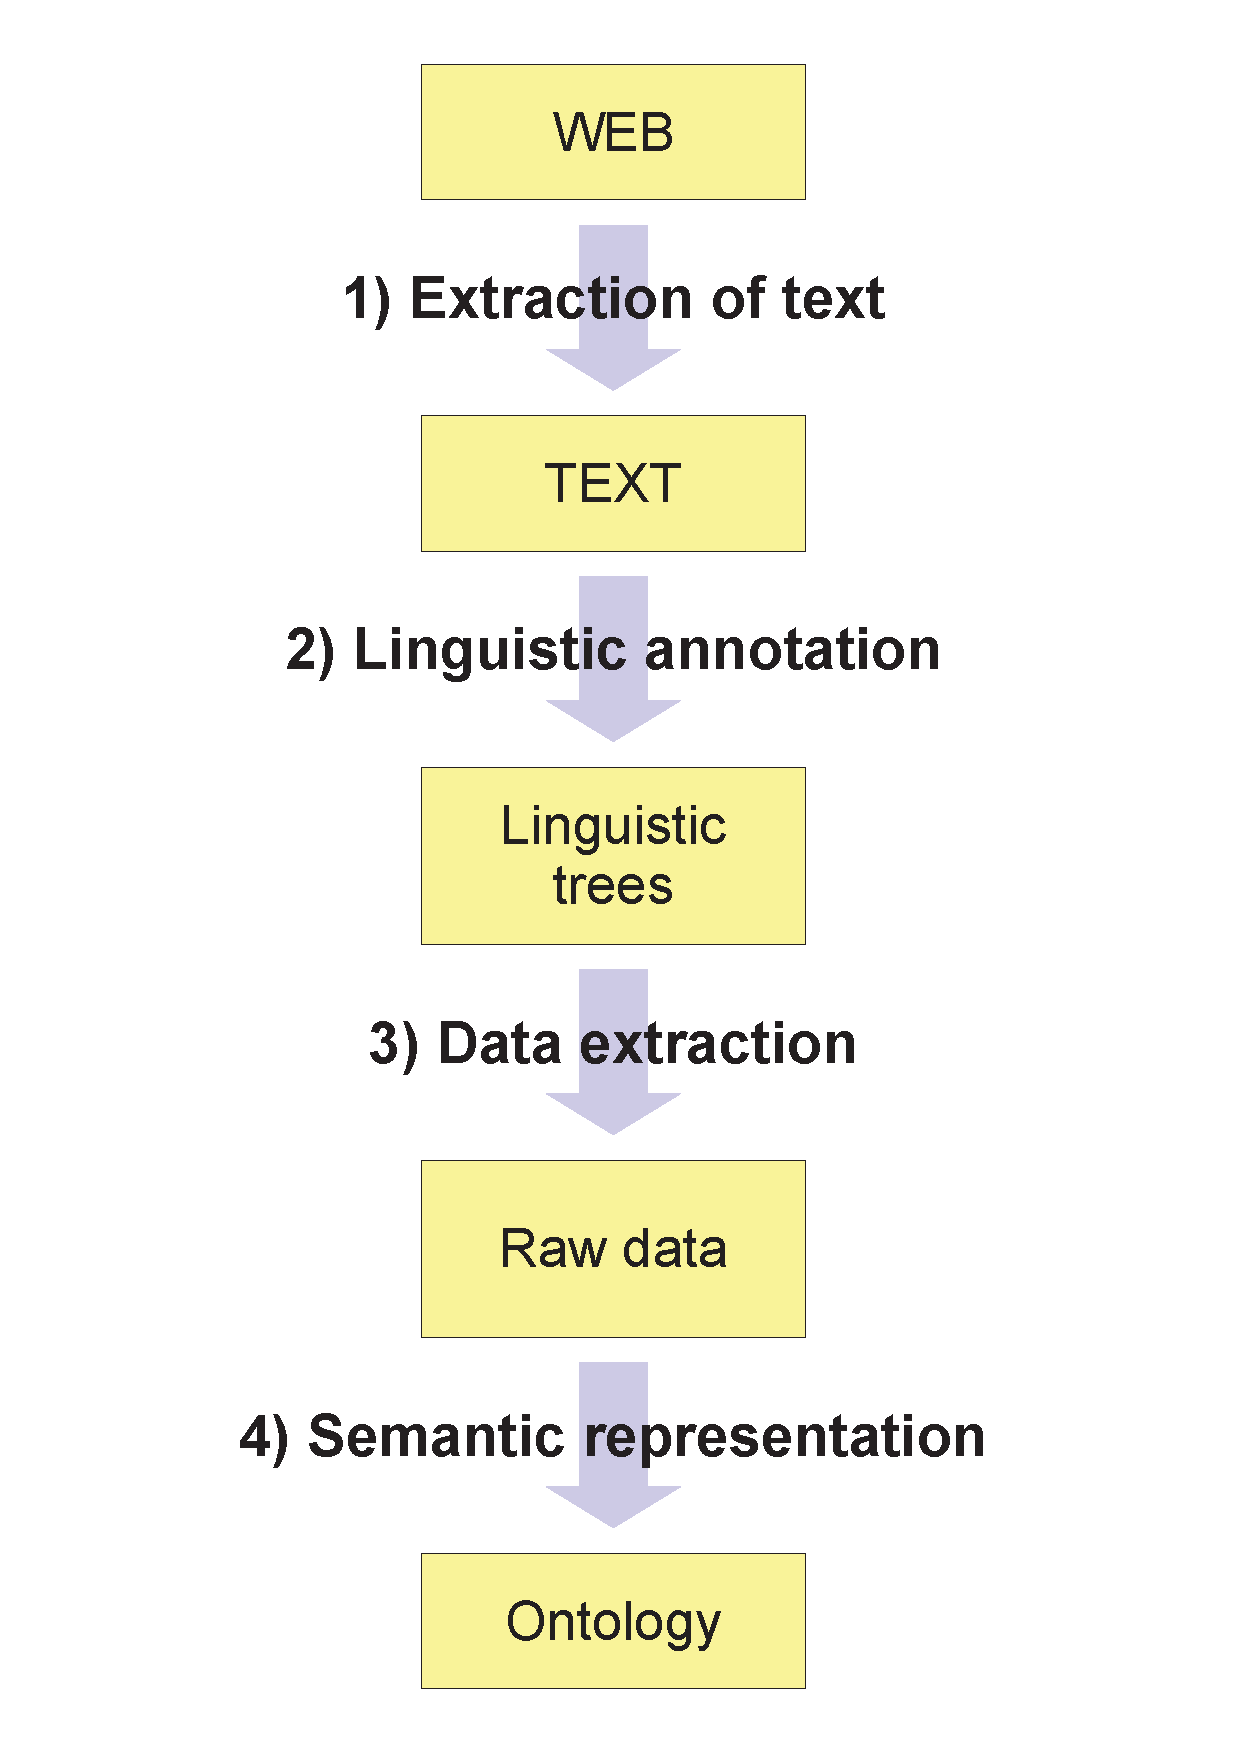
\includegraphics[width=0.2\hsize]{../img/ch3_ap_schema}
	\caption{Schema of the extraction process.}
	\label{fig:ch3_ap_schema}
\end{figure}


\begin{figure}
	\centering
		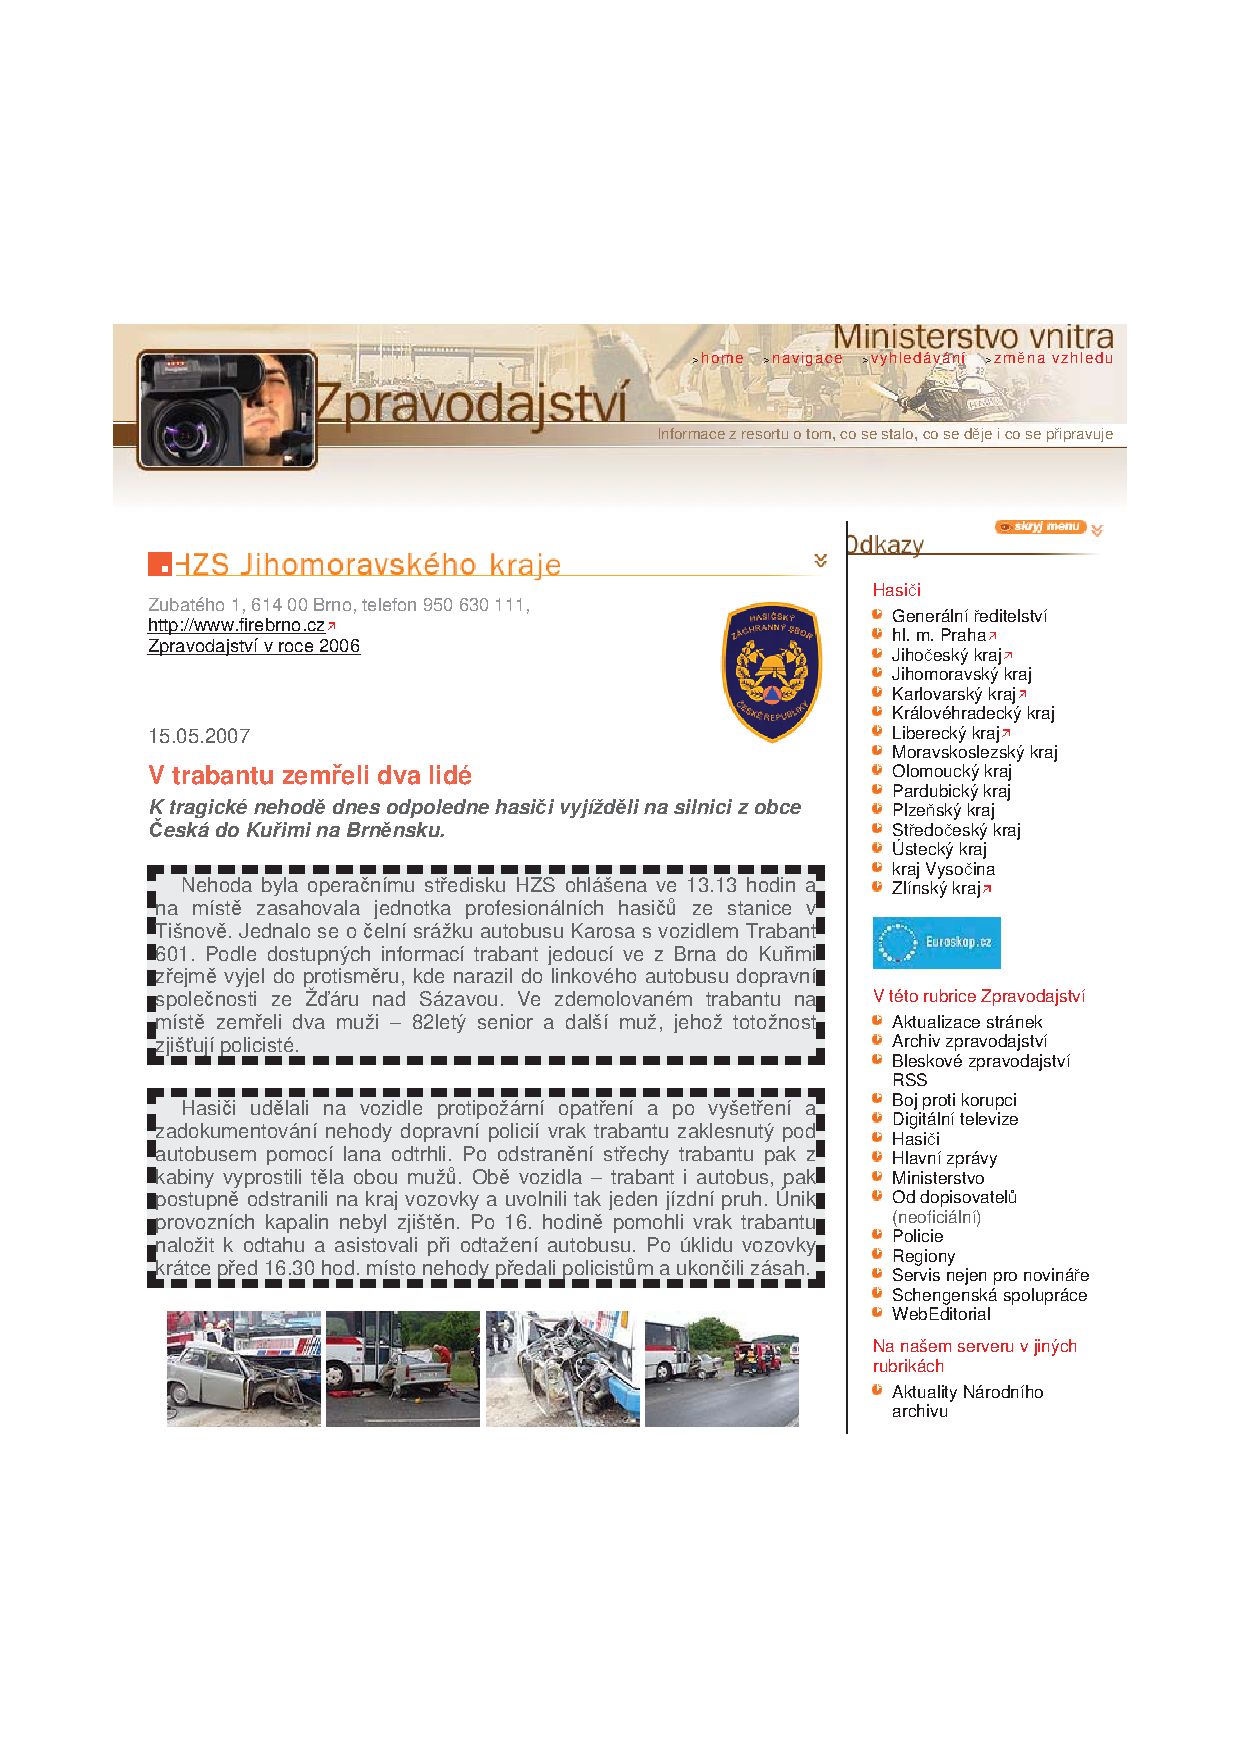
\includegraphics[width=0.5\hsize]{../img/ch3_article}
	\caption{One web page with an accident report.}
	\label{fig:ch3_article}
\end{figure}


\begin{figure}
	\centering
		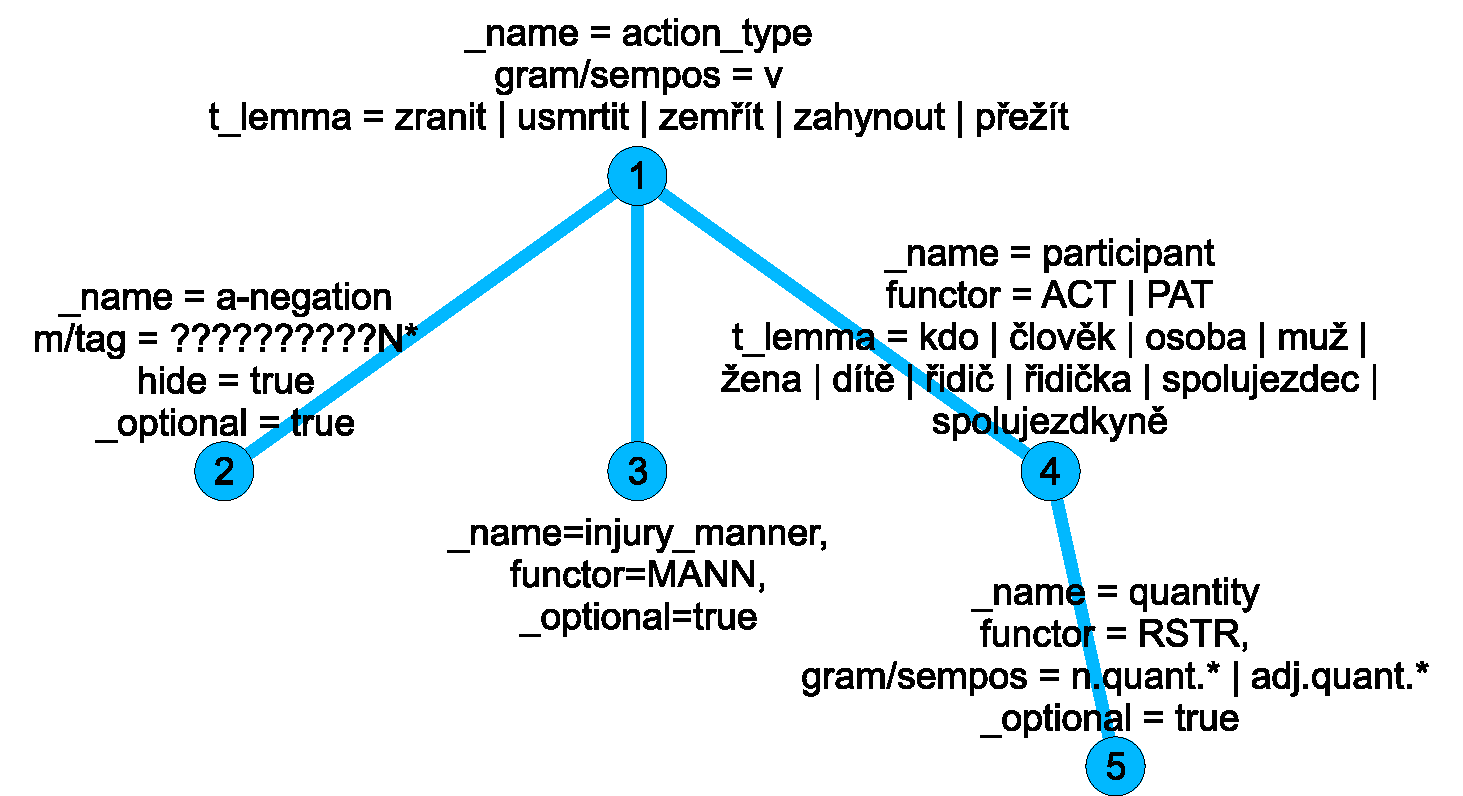
\includegraphics[width=0.5\hsize]{../img/ch3_extract_patern}		
\\Transcript:\\
\begin{tabular}{|c|c|c|c|c|}
\hline
zranit & usmrtit & zemřít & zahynout & přežít\\
to injure & to kill & to die & to wane & to survive\\
\hline
\end{tabular}
\\\begin{tabular}{|c|c|c|c|c|c|}
\hline
kdo & člověk & osoba & muž & žena & dítě\\
somebody & (hu)man & person & man & woman & child\\
\hline
\end{tabular}
\\\begin{tabular}{|c|c|c|c|}
\hline
řidič & řidička & spolujezdec & spolujezdkyně\\
driver & woman driver & passenger & woman passenger\\	
\hline
\end{tabular}		
	\caption{A manually created extraction rule investigating numbers of injuries and fatalities.}
	\label{fig:ch3_extract_patern}
\end{figure}

\begin{figure}
	\centering
		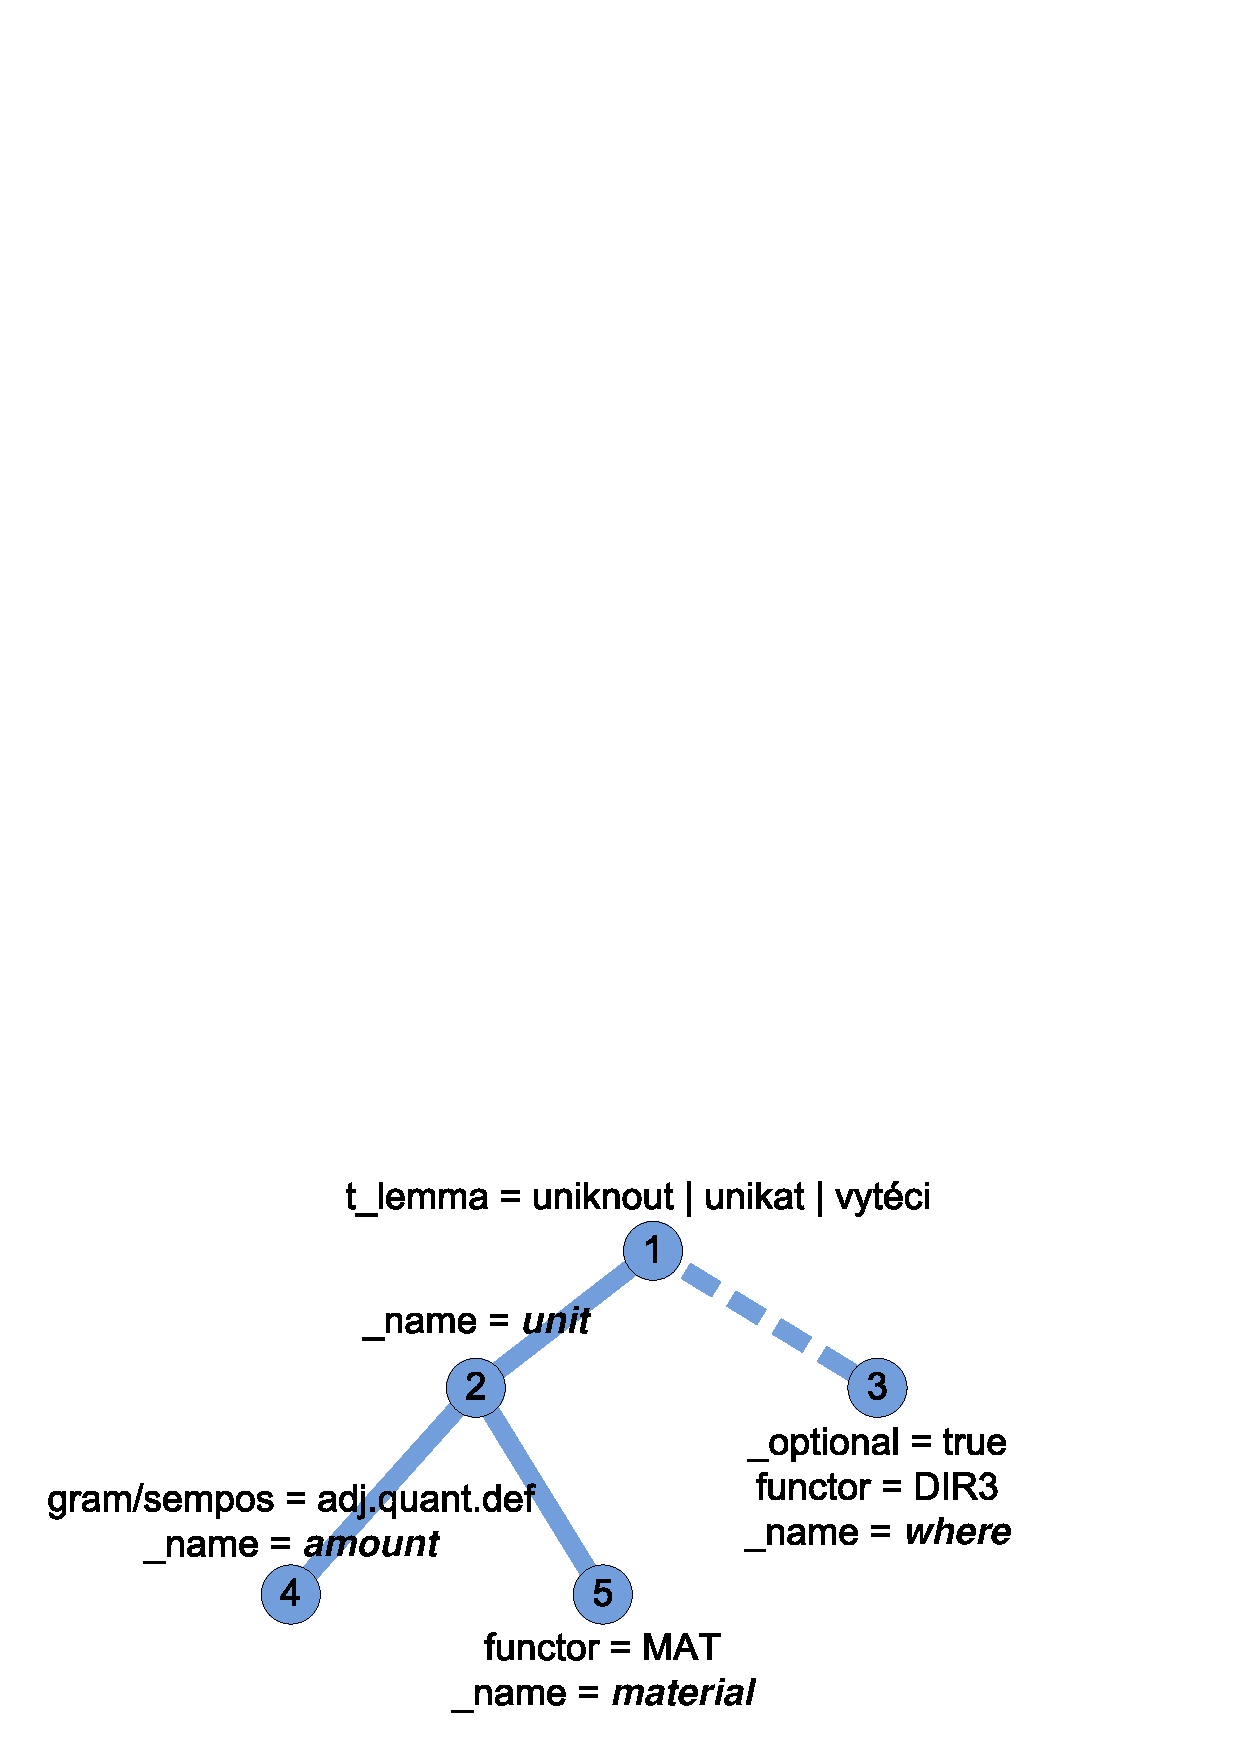
\includegraphics[width=0.5\hsize]{../img/ch3_eenv_extract_patern}
	\caption{A manually created extraction rule investigating dangerous liquids that spilled out into the environment.}
	\label{fig:ch3_eenv_extract_patern}
\end{figure}


\begin{figure}
	\centering
		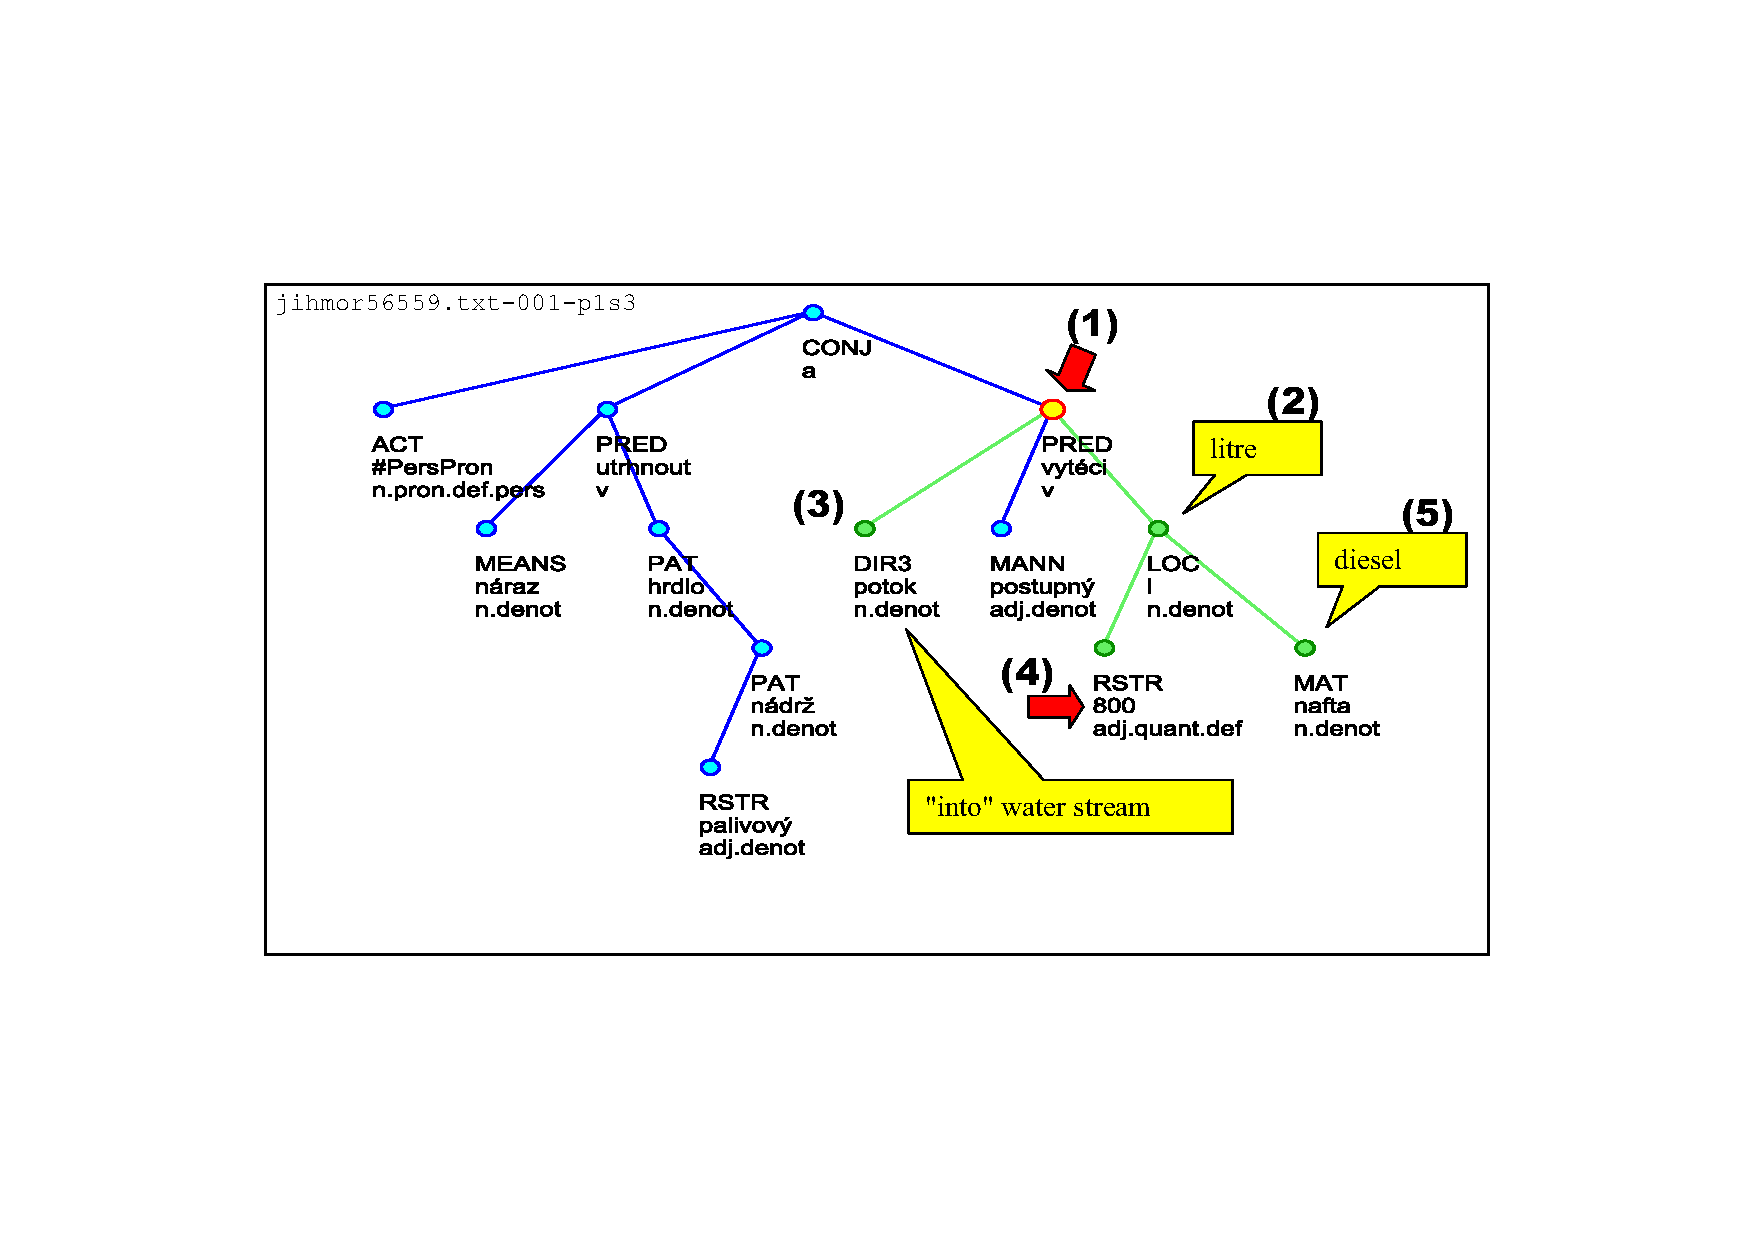
\includegraphics[angle=-90, width=0.6\hsize]{../img/ch3_eenv_matching_tree}
		
Original sentence: 
\emph{``Nárazem se utrhl hrdlo palivové nádrže a do potoka postupně vyteklo na 800 litrů nafty.''}\\
English transcript: 
\emph{``Due to the clash the throat of fuel tank tore off and 800 liters of oil (diesel) has run out to a stream.''}
	\caption{A tree matching with the corresponding extraction rule in Figure~\ref{fig:ch3_eenv_extract_patern}.}
	\label{fig:ch3_eenv_matching_tree}
\end{figure}


\begin{figure}
	\centering
		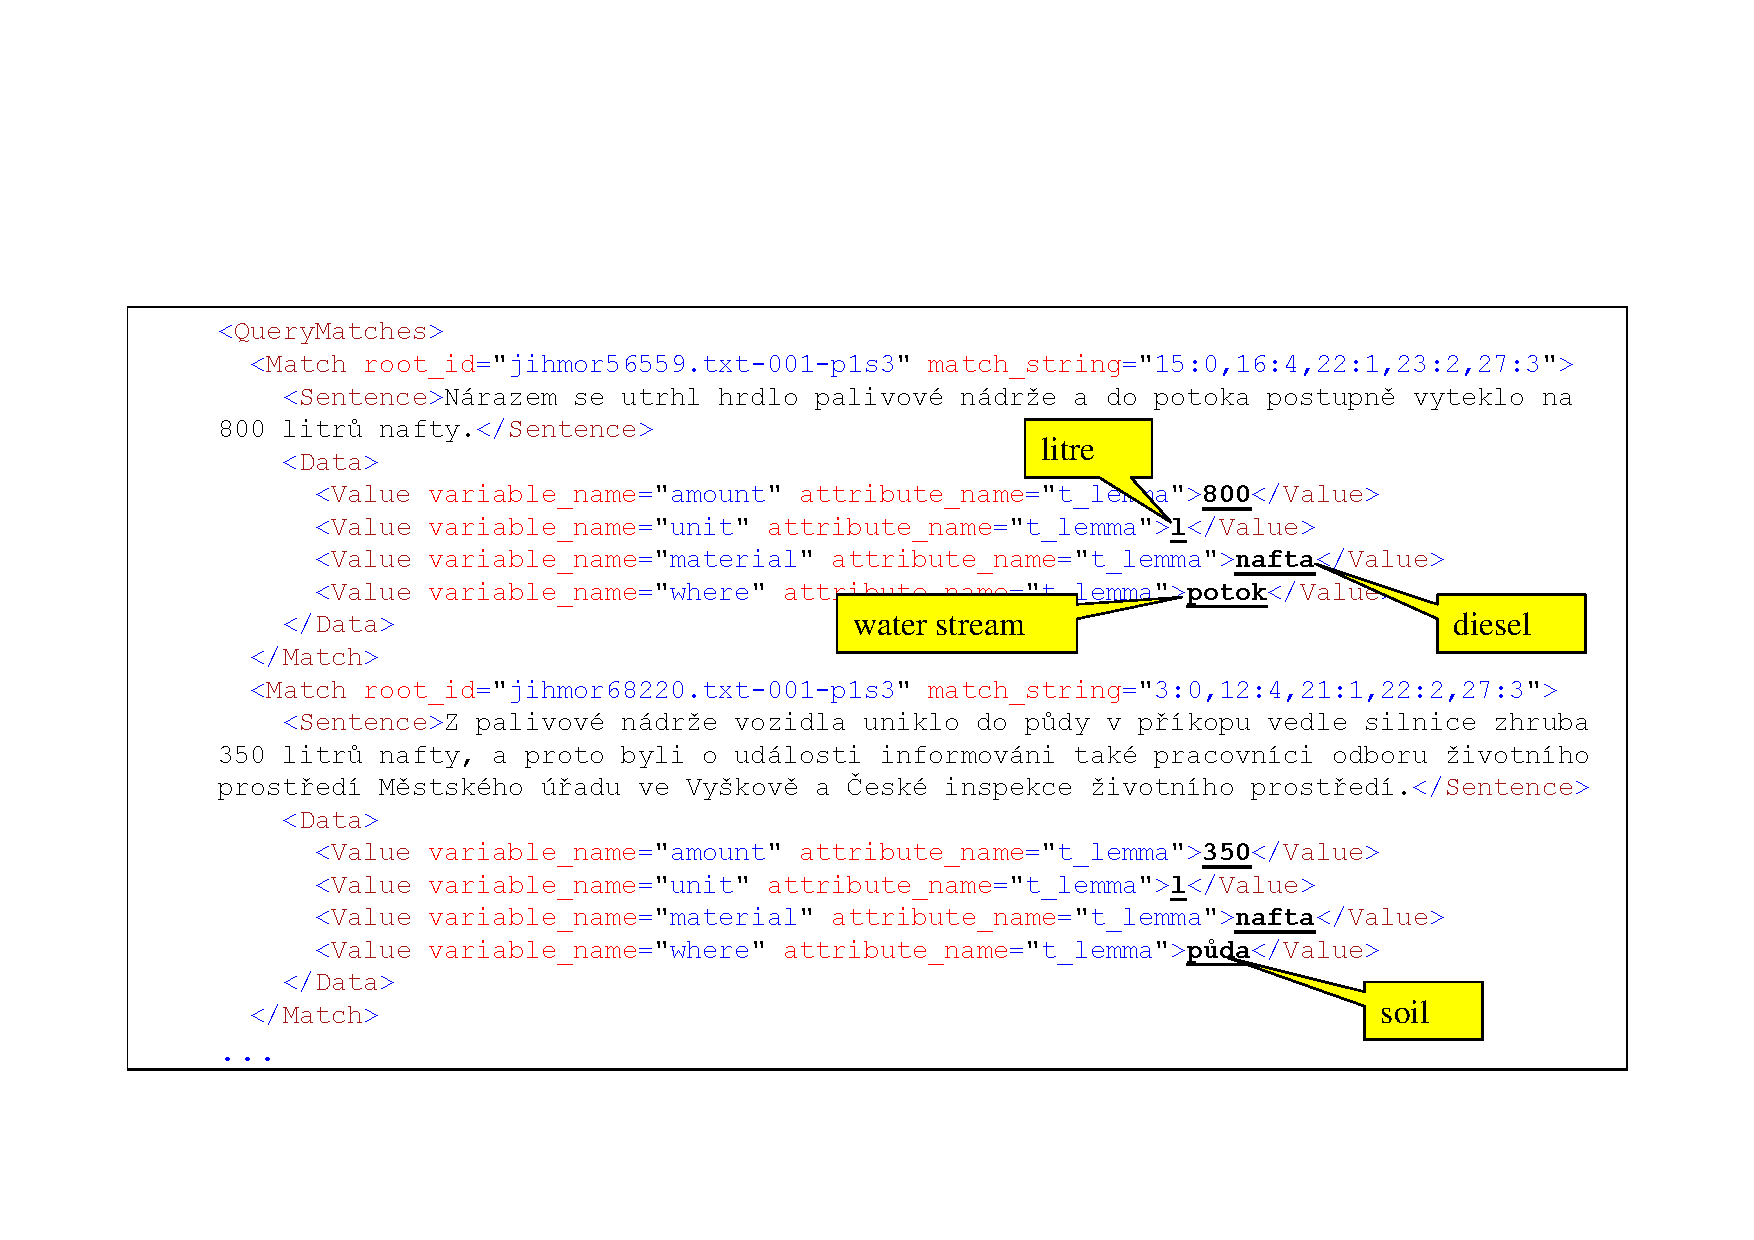
\includegraphics[angle=-90, width=0.7\hsize]{../img/ch3_eenv_results}
	\caption{\emph{XML} structured output of the SQL select like query corresponding with the extraction rule in Figure~\ref{fig:ch3_eenv_extract_patern} and matching tree in Figure~\ref{fig:ch3_eenv_matching_tree}.}
	\label{fig:ch3_eenv_results}
\end{figure}



\begin{figure}
	\centering
		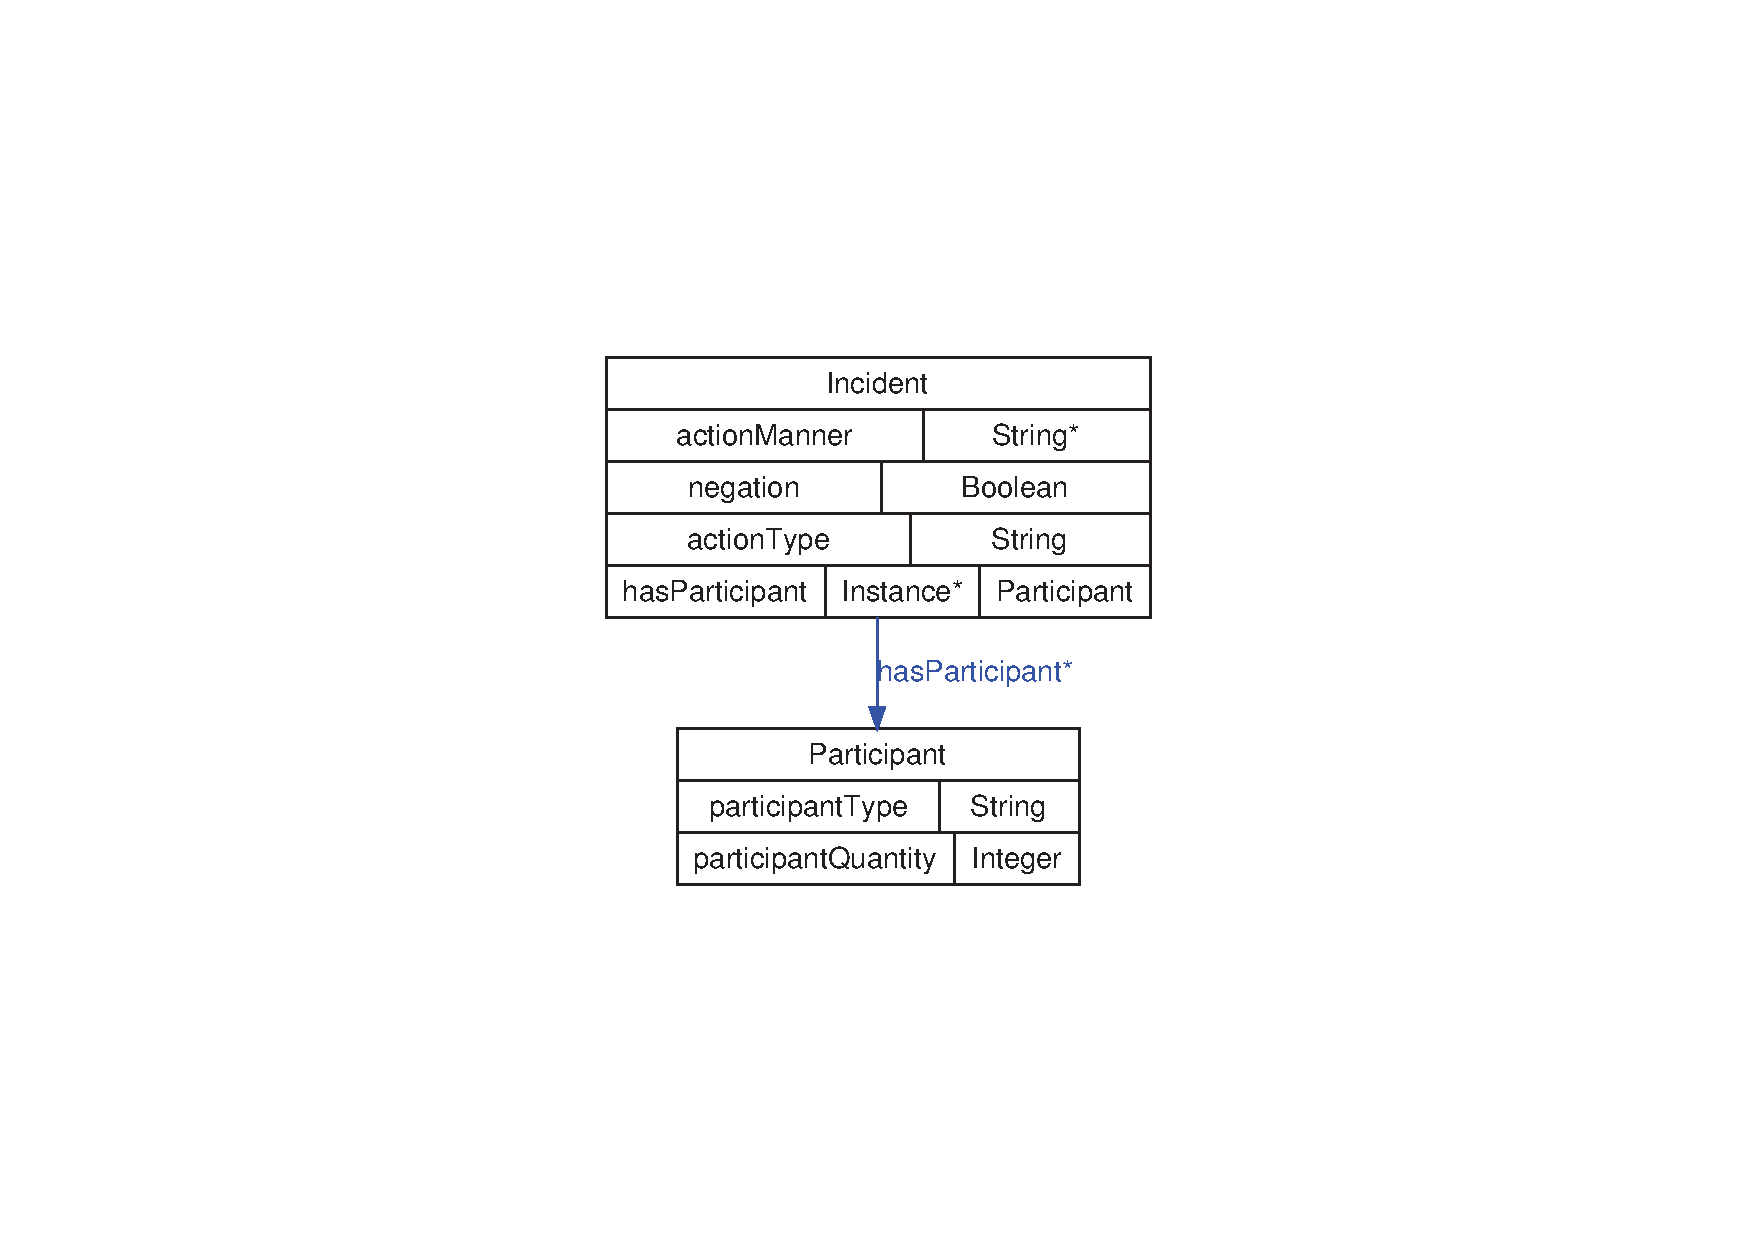
\includegraphics[angle=-90, width=0.3\hsize]{../img/ch3_classes}
	\caption{Schema of the target ontology.}
	\label{fig:ch3_classes}
\end{figure}


\begin{figure}
	\centering
		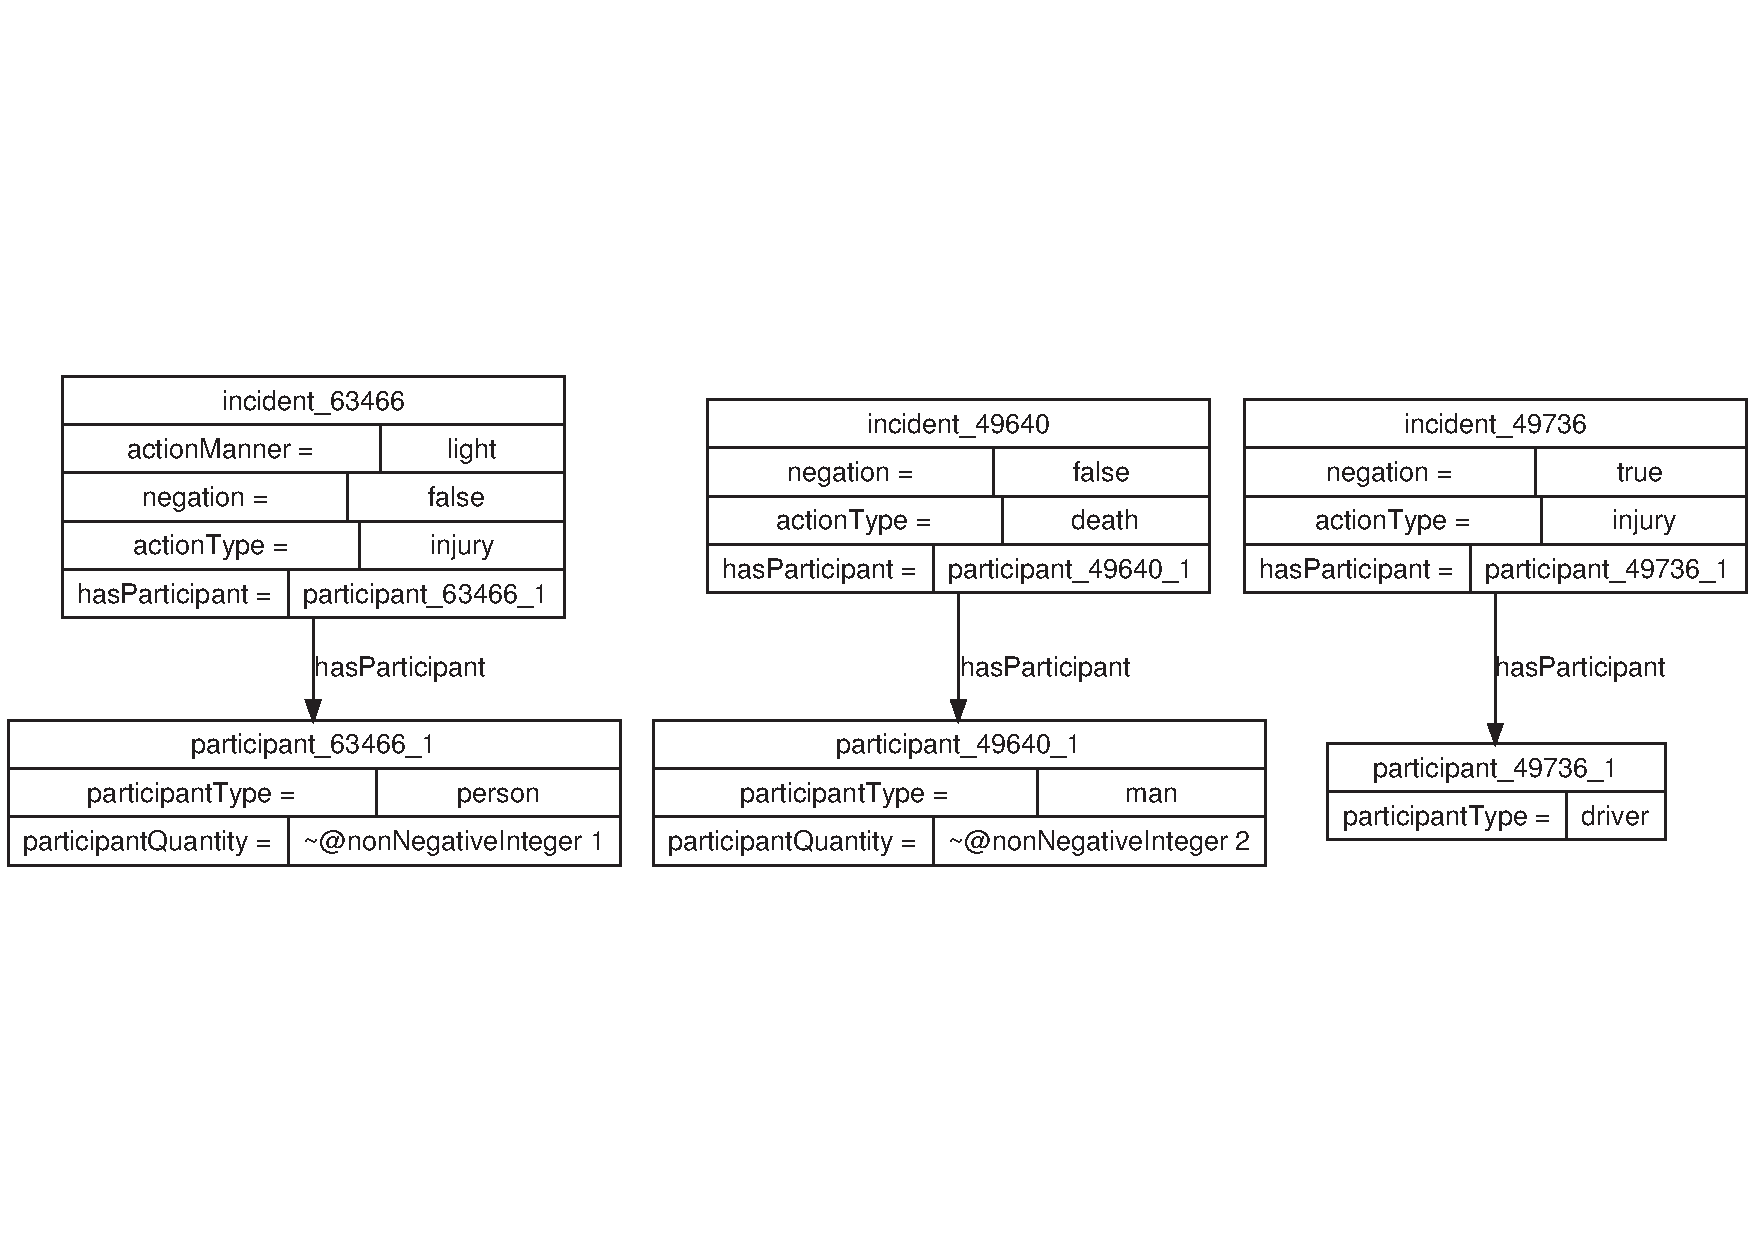
\includegraphics[angle=-90, width=\hsize]{../img/ch3_instances}
	\caption{Extracted instances of the target ontology.}
	\label{fig:instatnces}
\end{figure}


\begin{figure}
	\centering
		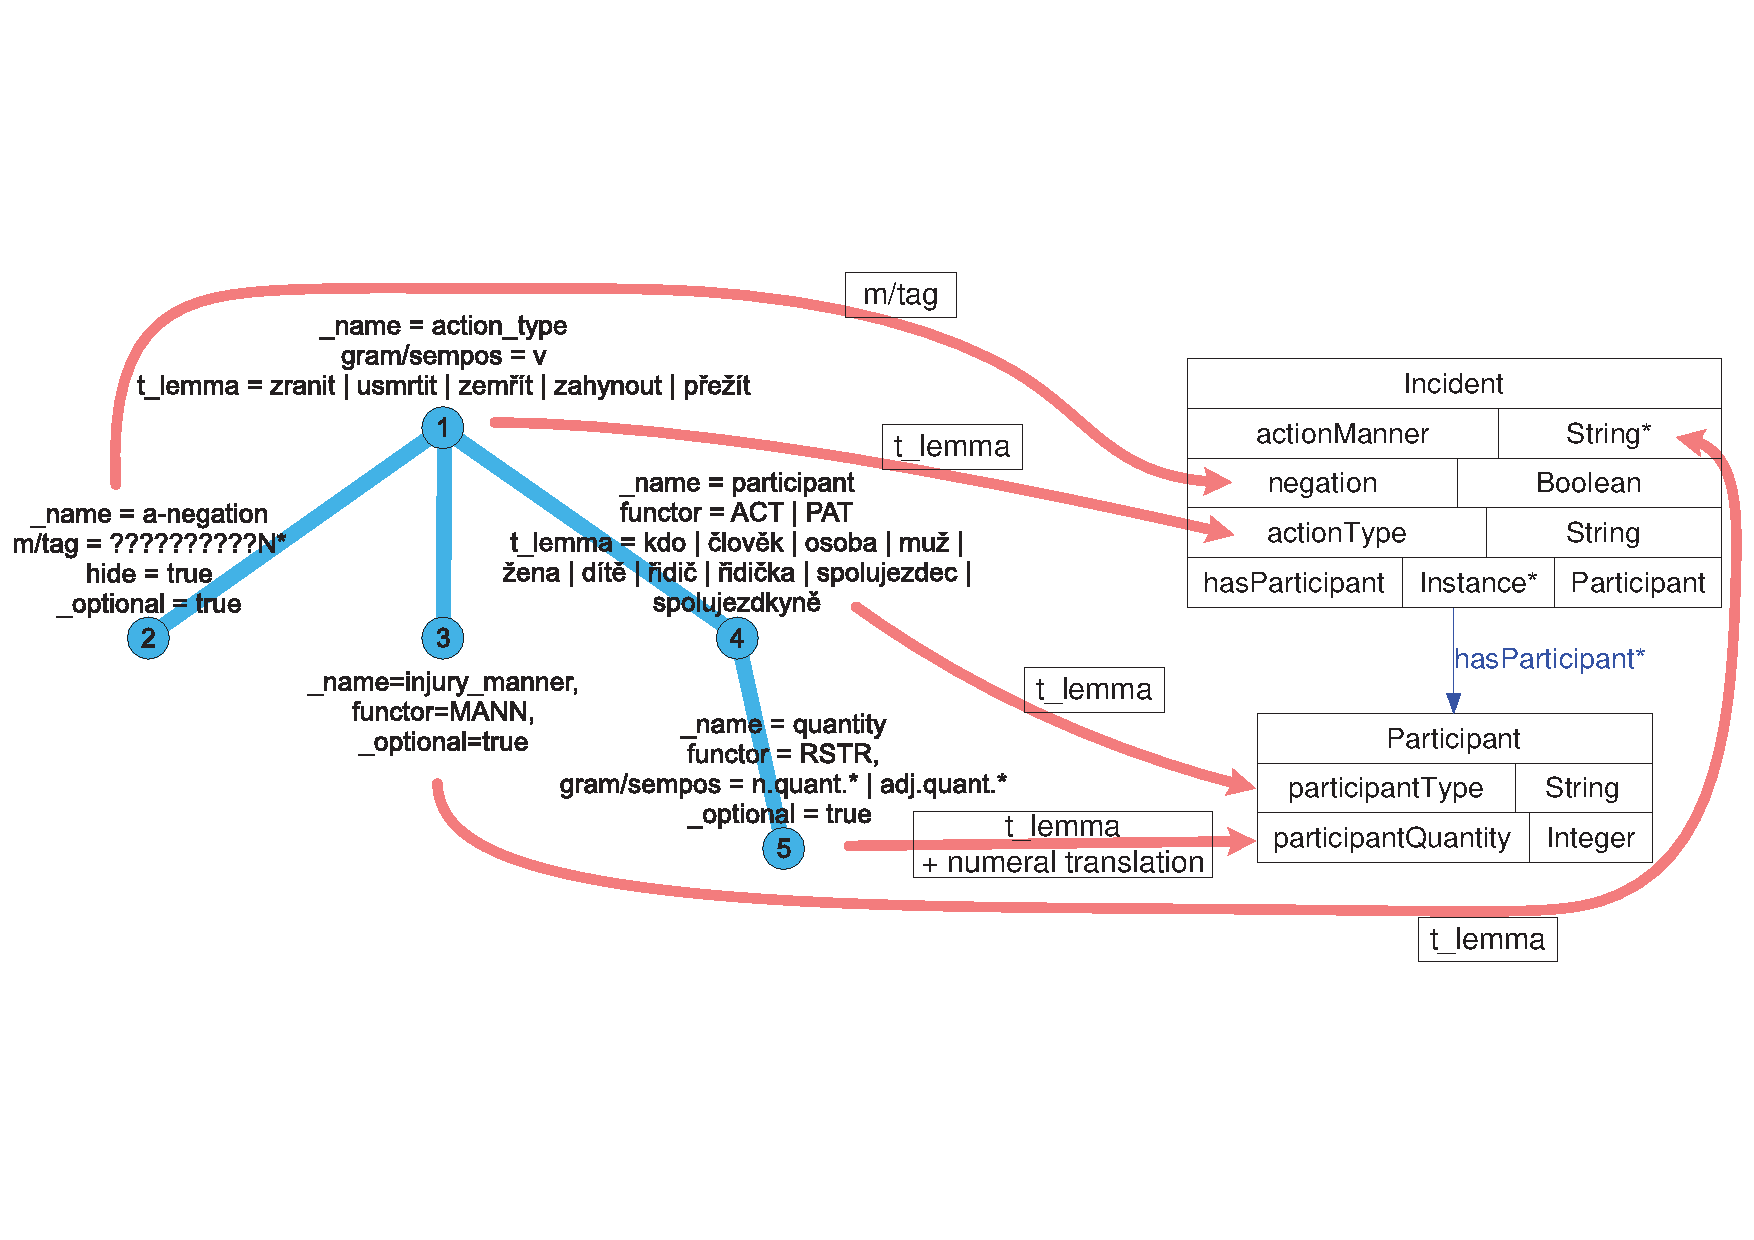
\includegraphics[angle=-90, width=0.9\hsize]{../img/ch3_semantic_interpretation}
	\caption{Semantic interpretation of the extraction rule.}
	\label{fig:ch3_semantic_interpretation}
\end{figure}


\begin{figure}
	\centering
		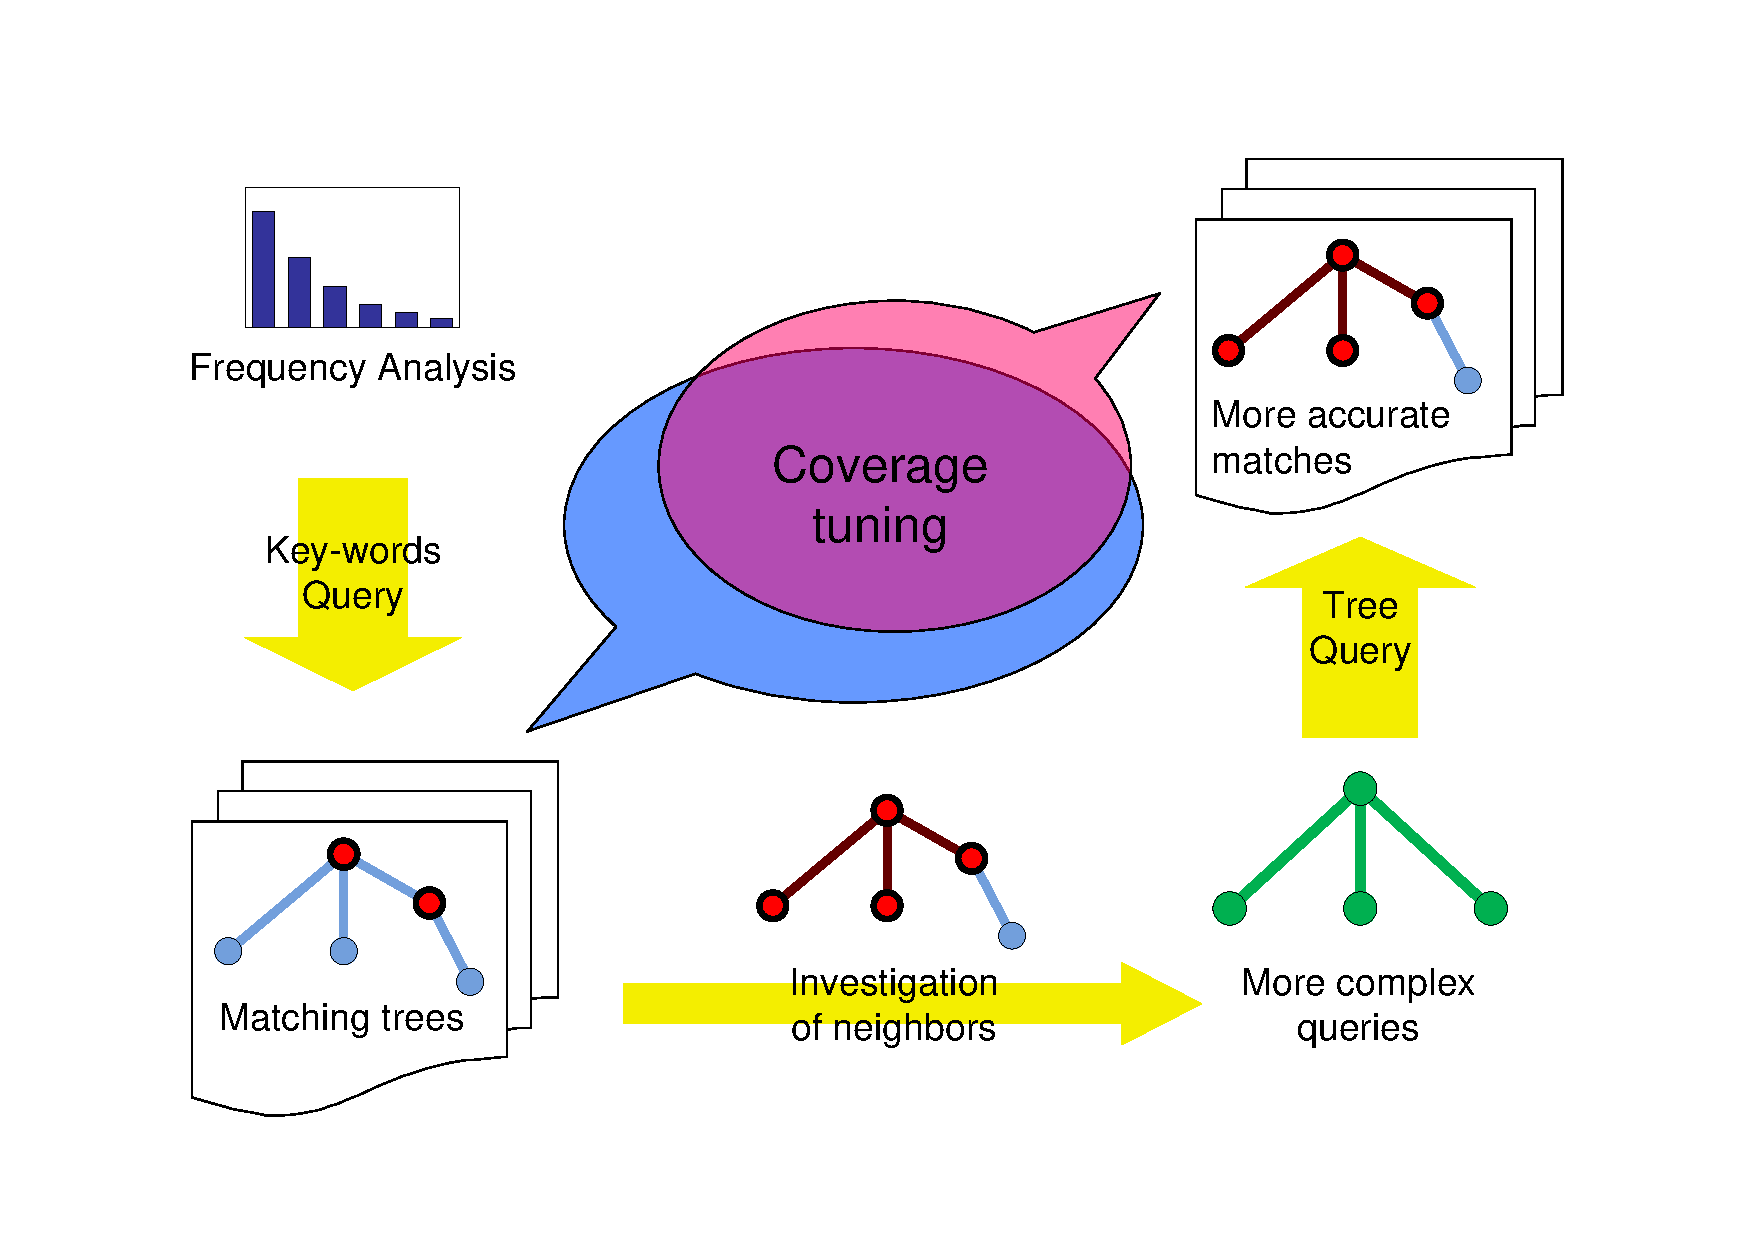
\includegraphics[angle=-90, width=0.5\hsize]{../img/ch3_coverge_tuning}
	\caption{Gradual refinement of an extraction rule.}
	\label{fig:ch3_coverge_tuning}
\end{figure}


\begin{figure}
\fbox{\parbox[b]{\hsize}{
\hspace*{0cm}$\bullet$ entita:1\\
\hspace*{1cm}$\bullet$ objekt:1\\
\hspace*{2cm}$\bullet$ celek:1\\
\hspace*{3cm}$\bullet$ artefakt:1, výtvor:2, výrobek:2\\
\hspace*{4cm}$\bullet$ vybavení:2\\
\hspace*{5cm}$\bullet$ přepravní prostředek:1, transportní prostředek:1\\
\hspace*{6cm}$\triangleright$ \textbf{veřejná doprava:1}\\
\hspace*{7cm}$\Rightarrow$ \emph{autobus:1, autokar:1}\\
\hspace*{6cm}$\triangleright$ \textbf{dopravní prostředek:1}\\
\hspace*{7cm}$\bullet$ kolové vozidlo:1\\
\hspace*{8cm}$\bullet$ samohybné vozidlo:1, vozidlo s vlastním pohonem:1\\
\hspace*{9cm}$\bullet$ motorové vozidlo:1\\
\hspace*{10cm}$\bullet$ nákladní automobil:1\\
\hspace*{11cm}$\Rightarrow$ \emph{kamion:1}

\vspace{1cm}

\setlength{\columnsep}{0cm}

\begin{multicols}{2}

\hspace*{0cm}$\bullet$ motorové vozidlo:1\\
\hspace*{1cm}$\bullet$ motocykl:1\\
\hspace*{1cm}$\bullet$ nákladní automobil:1\\
\hspace*{1cm}$\bullet$ obojživelné vozidlo:1\\
\hspace*{1cm}$\bullet$ auto:1, vůz:2\\
\hspace*{1cm}$\bullet$ pohřební vůz:1\\
\hspace*{1cm}$\bullet$ sněžný pluh:1, pluh:2\\
\hspace*{1cm}$\bullet$ golfový vozík:1\\

\vspace{0.5cm}

\hspace*{0cm}$\bullet$ nákladní automobil:1\\
\hspace*{1cm}$\bullet$ dodávka:3\\
\hspace*{1cm}$\bullet$ sklápěč:1, vyklápěcí nákladní automobil:1\\
\hspace*{1cm}$\bullet$ tahač:1\\
\hspace*{1cm}$\bullet$ pick-up:1, malý nákladní automobil:1\\
\hspace*{1cm}$\bullet$ hasící vůz:1, požární stříkačka:1\\
\hspace*{1cm}$\bullet$ rozhlasový vůz:1\\
\hspace*{1cm}$\bullet$ kamion:1\\
\hspace*{1cm}$\bullet$ nákladní automobil s přívěsem:1\\
\hspace*{1cm}$\bullet$ popelářský vůz:1, popelářské auto:1, bobr:3\\

\columnbreak

\hspace*{0cm}$\bullet$ auto:1, vůz:2\\
\hspace*{1cm}$\bullet$ limuzína:1\\
\hspace*{1cm}$\bullet$ elektrický vozík:1\\
\hspace*{1cm}$\bullet$ závodní vůz:1, závodní automobil:1\\
\hspace*{1cm}$\bullet$ sportovní vůz:1\\
\hspace*{1cm}$\bullet$ kabriolet:1, sporťák:1\\
\hspace*{1cm}$\bullet$ vrak:3\\
\hspace*{1cm}$\bullet$ limuzína:2\\
\hspace*{1cm}$\bullet$ hlídkový vůz:1, policejní vůz:1\\
\hspace*{1cm}$\bullet$ sériový automobil:1\\
\hspace*{1cm}$\bullet$ cestovní vůz:1\\
\hspace*{1cm}$\bullet$ džíp:1\\
\hspace*{1cm}$\bullet$ kupé:1\\
\hspace*{1cm}$\bullet$ kabriolet:3\\
\hspace*{1cm}$\bullet$ kombi:1\\
\hspace*{1cm}$\bullet$ taxi:1\\
\hspace*{1cm}$\bullet$ ambulance:1, sanitka:1, pohotovost:6,\\
\hspace*{2cm} záchranka:1, sanita:1
\end{multicols}
\setlength{\columnsep}{5cm}
}}
	\caption{Sample of Czech WordNet showing the word coverage in the domain of means of transport and vehicles.}
	\label{fig:chX_czWordNet}
\end{figure}



\section{Listings}

\begin{listing}[ht]
\begin{minted}[linenos,  fontsize=\footnotesize,
               frame=lines]{perl}

my @injure_verbs = ("zranit", "usmrtit", "zemřít", "zahynout", "přežít");

sub print_injured {
	if ($this->{gram}{sempos} eq "v") {
		foreach my $v (@injure_verbs) {
			if ($this->{t_lemma} eq $v ) {
				#action type
				print "<action type=\"" . $this->{t_lemma} . "\">";

				#sentece
				print "<sentece>" . PML_T::GetSentenceString($root) . "</sentece>";
				print "<sentece_id>" . $root->{id} . "</sentece_id>";
				
				#negation
				if (test_negation($this)) {
					print "<negation>true</negation>" ;					
				} else {
					print "<negation>false</negation>" ;										
				}
								
				#manner of injurance
				my @mans = find_node_by_attr_depth($this, 0, 'functor', '^MANN');
				if (@mans) {
					foreach my $m (@mans) {
						print "<manner>"; 
						print $m->{t_lemma};
						print "</manner>"; 
					};
				}
				
				#actors and patients
				my @pats = find_node_by_attr($this, 'functor', '^[PA][AC]T');
				@pats = &filter_list(\&test_person, @pats);
				
				foreach my $p (@pats) {
					print "<participant type=\"" . $p->{t_lemma} . "\">";

					#patients count
					my @cnt = find_node_by_attr($p, 'functor', '^RSTR');
					@cnt = &filter_list(\&test_number_lemma, @cnt);
					my $cnt1 = pop(@cnt);
					print "<quantity>" . 
						&test_number($cnt1->{t_lemma}) . 
						"</quantity>" if ($cnt1);
	
					print "<full_string>";
					print_subtree_as_text($p);
					print "</full_string>";

					print "</participant>";
				}
				
				#action end
				print "</action>\n";											
}}}}
\end{minted}
\caption{Procedurally written extraction rule in \emph{Btred}.}
\label{lst:btred_rule}
\end{listing}
%%%%%%%%%%%%%%%%%%%%%%%%%%%%%%%%%%%%%%%%%%%%%%%%%%%%%%%%%%%%%%%%%%%%%%%%%%%%%%%%%%%%%



%%%%%%%%%%%%%%%%%%%%%%%%%%%%%%%%%%%%%%%%%%%%%%%%%%%%%%%%%%%%%%%%%%%%%%%%%%%%%%%%%%%%%
\begin{listing}[ht]
\begin{minted}[linenos,  fontsize=\footnotesize,
               frame=lines]{sparql}

SELECT ?action ?participant ?participant_type ?quantity
WHERE {
	{
		?action rdf:type :Incident;
			:actionType "death";
			:negation false.
	} UNION {
		?action rdf:type :Incident;
			:actionType "survival";
			:negation true.
	}
	?action :hasParticipant ?participant.
	?participant :participantType ?participant_type.
	OPTIONAL {
		?participant :participantQuantity ?quantity.
	}
}
\end{minted}
\caption{\emph{SPARQL} query that summarizes fatalities of particular incidents.}
\label{lst:sparql_aggregation}
\end{listing}
%%%%%%%%%%%%%%%%%%%%%%%%%%%%%%%%%%%%%%%%%%%%%%%%%%%%%%%%%%%%%%%%%%%%%%%%%%%%%%%%%%%%%



%%%%%%%%%%%%%%%%%%%%%%%%%%%%%%%%%%%%%%%%%%%%%%%%%%%%%%%%%%%%%%%%%%%%%%%%%%%%%%%%%%%%%
\begin{listing}[ht]
\begin{minted}[linenos,  fontsize=\footnotesize,
               frame=lines]{xml}
<injured_result>
	<action type="zranit">
		<sentece>
			Při požáru byla jedna osoba lehce zraněna -- jednalo se
			o majitele domu, který si vykloubil rameno.
		</sentece>
		<sentece_id>T-vysocina63466.txt-001-p1s4</sentece_id>
		<negation>false</negation>
		<manner>lehký</manner>
		<participant type="osoba">
			<quantity>1</quantity>
			<full_string>jedna osoba</full_string>
		</participant>
	</action>
	<action type="zemřít">
		<sentece>
			Ve zdemolovaném trabantu na místě zemřeli dva muži -- 82letý
			senior a další muž, jehož totožnost zjišťují policisté.
		</sentece>
		<sentece_id>T-jihomoravsky49640.txt-001-p1s4</sentece_id>
		<negation>false</negation>
		<participant type="muž">
			<quantity>2</quantity>
			<full_string>dva muži</full_string>
		</participant>
	</action>
		<action type="zranit">
		<sentece>čtyřiatřicetiletý řidič nebyl zraněn.</sentece>
		<sentece_id>T-jihomoravsky49736.txt-001-p4s3</sentece_id>
		<negation>true</negation>
		<participant type="řidič">
			<full_string>čtyřiatřicetiletý řidič</full_string>
		</participant>
	</action>
</injured_result>
\end{minted}
\caption{\emph{XML} structured output of the query written in \emph{Btred}.}
\label{lst:btred_xml}
\end{listing}
%%%%%%%%%%%%%%%%%%%%%%%%%%%%%%%%%%%%%%%%%%%%%%%%%%%%%%%%%%%%%%%%%%%%%%%%%%%%%%%%%%%%%




%%%%%%%%%%%%%%%%%%%%%%%%%%%%%%%%%%%%%%%%%%%%%%%%%%%%%%%%%%%%%%%%%%%%%%%%%%%%%%%%%%%%%
\begin{listing}[ht]
\begin{minted}[linenos,  fontsize=\footnotesize,
               frame=lines]{xml}
<QueryMatches>
	<Match root_id="T-vysocina63466.txt-001-p1s4" match_string="2:0,7:3,8:4,11:2">
		<Sentence>
			Při požáru byla jedna osoba lehce zraněna - jednalo se
			o majitele domu, který si vykloubil rameno.
		</Sentence>
		<Data>
			<Value variable_name="action_type" attribute_name="t_lemma">zranit</Value>
			<Value variable_name="injury_manner" attribute_name="t_lemma">lehký</Value>
			<Value variable_name="participant" attribute_name="t_lemma">osoba</Value>
			<Value variable_name="quantity" attribute_name="t_lemma">jeden</Value>
		</Data>
	</Match>
	<Match root_id="T-jihomoravsky49640.txt-001-p1s4" match_string="1:0,13:3,14:4">
		<Sentence>
			Ve zdemolovaném trabantu na místě zemřeli dva muži - 82letý senior
			a další muž, jehož totožnost zjišťují policisté.
		</Sentence>
		<Data>
			<Value variable_name="action_type" attribute_name="t_lemma">zemřít</Value>
			<Value variable_name="participant" attribute_name="t_lemma">muž</Value>
			<Value variable_name="quantity" attribute_name="t_lemma">dva</Value>
		</Data>
	</Match>
	<Match root_id="T-jihomoravsky49736.txt-001-p4s3" match_string="1:0,3:3,7:1">
		<Sentence>Čtyřiatřicetiletý řidič nebyl zraněn.</Sentence>
		<Data>
			<Value variable_name="action_type" attribute_name="t_lemma">zranit</Value>
			<Value variable_name="a-negation" 
			       attribute_name="m/tag">VpYS---XR-NA---</Value>
			<Value variable_name="participant" attribute_name="t_lemma">řidič</Value>
		</Data>
	</Match>
</QueryMatches>
\end{minted}
\caption{\emph{XML} structured output of the SQL select like query. A negation can be detected from the presence of \emph{m/tag} on the line 30.}
\label{lst:select_xml}
\end{listing}
%%%%%%%%%%%%%%%%%%%%%%%%%%%%%%%%%%%%%%%%%%%%%%%%%%%%%%%%%%%%%%%%%%%%%%%%%%%%%%%%%%%%%


\end{comment}


%%%%%%%%%%%%%%%%%%%%%%%%%%%%%%%%%%%%%%%%%%%%%%%%%%%%%%%%%%%%%%%%%%%%%%%%%%%%%%%%%%%%%
\begin{listing}[ht]
\begin{minted}[linenos,  fontsize=\footnotesize,
               frame=lines]{prolog}
serialize_rule_file(RuleFileName, OutputFileName, OntologyURI, ObjectProperties) :-
	assert(objectProperties(ObjectProperties)),
	open(OutputFileName, 'write', Stream), set_output(Stream),
	write('<?xml version="1.0" encoding="UTF-8"?>\n'),
	write('<!DOCTYPE Ontology [ <!ENTITY xsd "http://www.w3.org/2001/XMLSchema#" >\n'),
	write('	<!ENTITY pml "http://ufal.mff.cuni.cz/pdt/pml/" > ]>\n'),		
	write('<Ontology xmlns="http://www.w3.org/2002/07/owl#"\n'),	
	format('	ontologyIRI="~a">\n',[OntologyURI]),
	consult(RuleFileName),   %Each rule in the file will be processed by serialize_rule,
	                         %because of the term_expansion setting on the last line. 	                         
	write('</Ontology>'),			
	close(Stream).

serialize_rule(:-(H, B)) :- 	
	numbervars(:-(H, B), 0, _),	
	write('<DLSafeRule>\n'),		
		write('<Body>\n'),          
			serialize_term(B),                       %Rule body
		write('\n</Body>\n'), write('<Head>\n'),
			serialize_term(H),                       %Rule head
		write('\n</Head>\n'),			
	write('</DLSafeRule>\n\n'),!.
	 
%Serialize object property
serialize_term(T):- functor(T,F,N), objectProperties(OProps), member(F, OProps),!,	
	write('<ObjectPropertyAtom>'),
	format('<ObjectProperty IRI="&pml;~a"/>\n', [F]),
	serialize_arg(T, 0, N),		
	write('</ObjectPropertyAtom>').

%Serialize datatype property
serialize_term(T):- functor(T,F,N),	
	write('<DataPropertyAtom>'),
	format('<DataProperty IRI="&pml;~a"/>\n', [F]),
	serialize_arg(T, 0, N),		
	write('</DataPropertyAtom>').

%Serialize argument list
serialize_term(','(A,B)):- serialize_term(A), write('\n'), serialize_term(B),!.

%Serialize variable
serialize_term('$VAR'(N)):- char_code('a',I), Var is I + N,
	format('<Variable IRI="urn:swrl#~c"/>\n',[Var]),!.
%Serialize simple atom or string (printed without quotes)
serialize_term(T):- atom(T), format('<Literal>~a</Literal>\n',[T]),!.
%Serialize number
serialize_term(T):- simple(T), format('<Literal>~k</Literal>\n',[T]),!.

%Serialize term arguments: serialize_arg(+Term, +CurrentArgNumber, +LastArgNumber)
serialize_arg(T, _, 0).
serialize_arg(T, N, N).
serialize_arg(T, M, N) :-  M2 is M+1, arg(M2, T, A),
	serialize_term(A), serialize_arg(T, M2, N).  
                                                  %All predicates loaded by consult
term_expansion(T,T):- serialize_rule(T).          %will be processed by serialize_rule.
\end{minted}
\caption{Prolog module for export of extraction rules to OWL XML.}
\label{lst:rules_export}
\end{listing}
%%%%%%%%%%%%%%%%%%%%%%%%%%%%%%%%%%%%%%%%%%%%%%%%%%%%%%%%%%%%%%%%%%%%%%%%%%%%%%%%%%%%%


\begin{comment}

\clearpage

\subsection{Evaluation}



\begin{table}
	\centering
		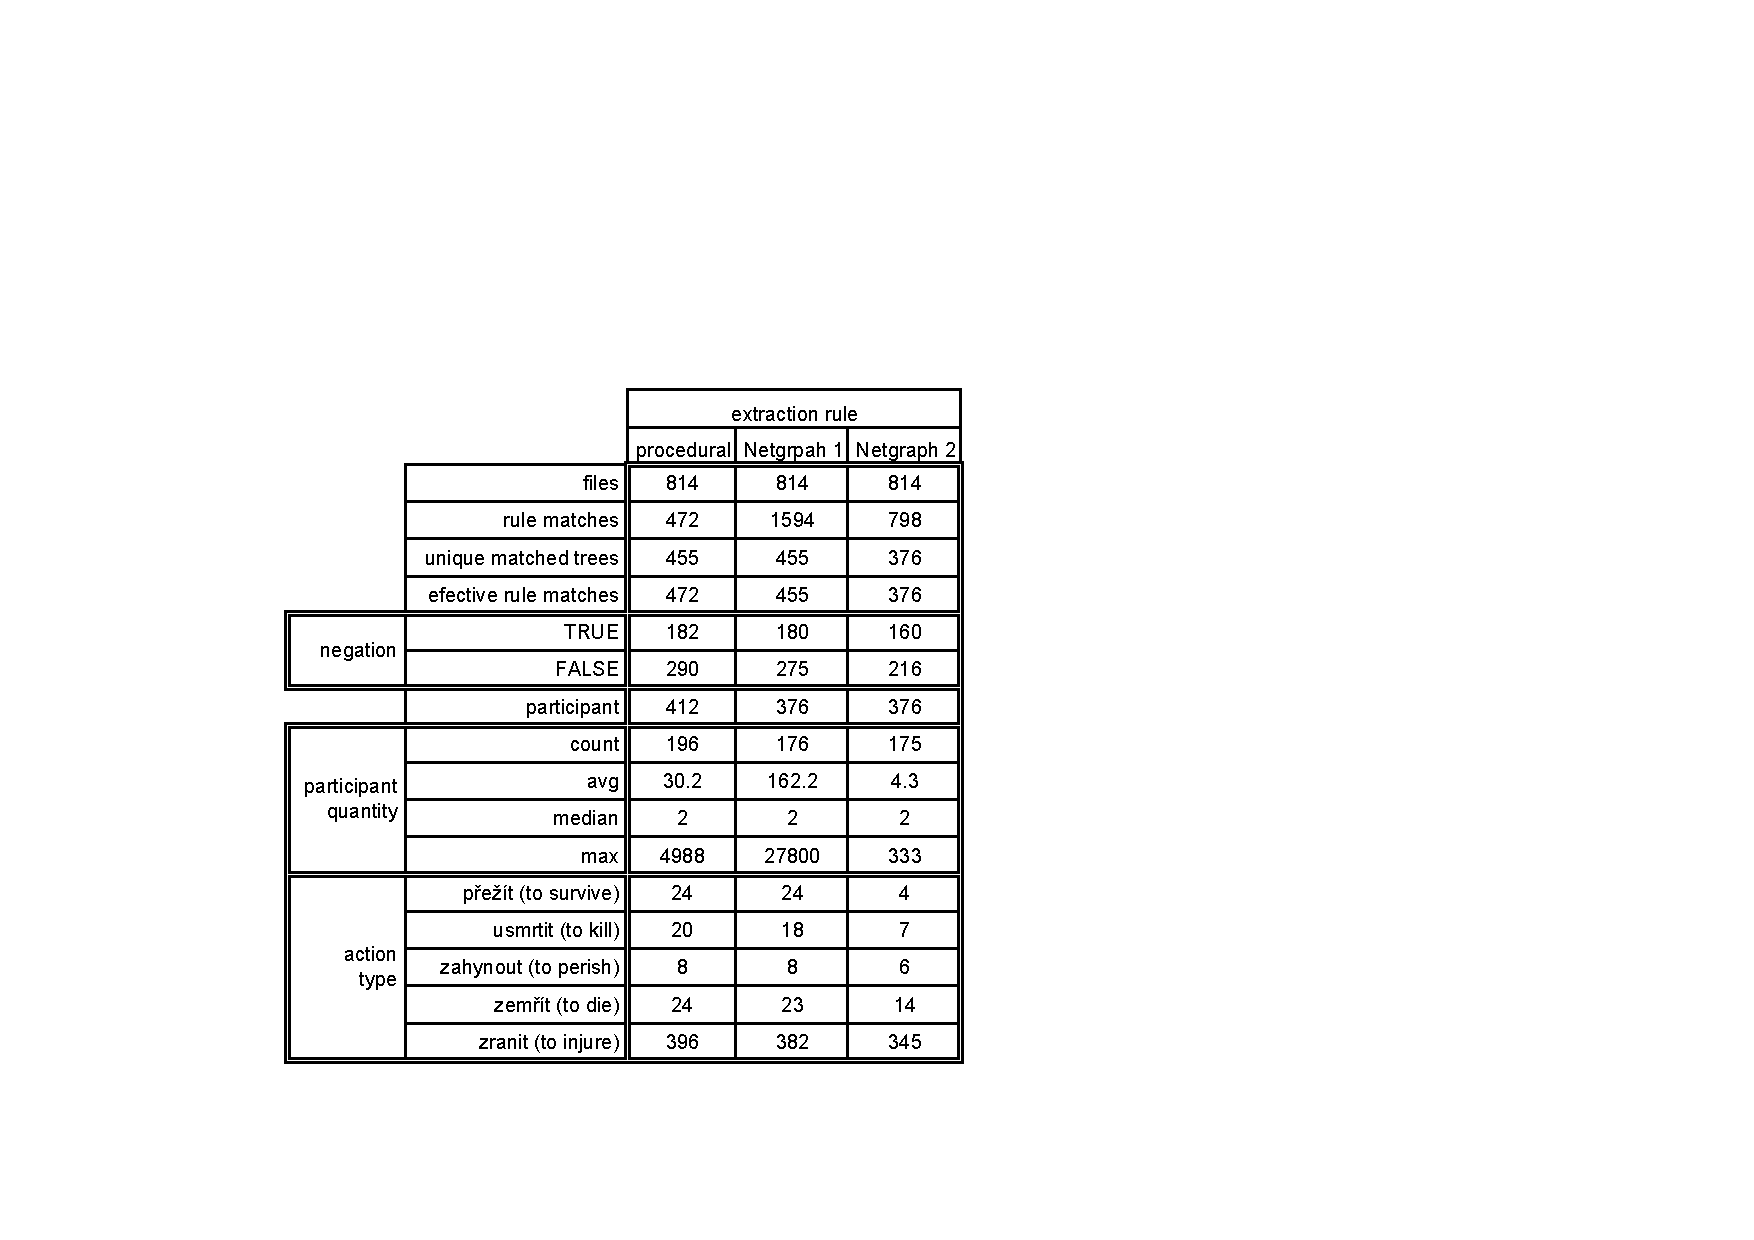
\includegraphics[angle=-90,width=0.6\hsize]{../img/ch3_tab_manual_rules}
	\caption{Evaluation of manually created rules (bigger dataset without manual annotations).}
	\label{tab:ch3_tab_manual_rules}
\end{table}



\begin{table}
	\centering
	\begin{tabular}{|r|c|c|c|c|c|c|}
		\hline
		 & correct & missing & spurious & recall & precision & $F_1$\\
		\hline
		injuries & 3 & 29 & 0 & 0.09 & 1 & 0.17\\
		\hline
		fatalities & 1 & 10 & 0 & 0.09 & 1 & 0.17\\
		\hline
	\end{tabular}
	\caption{Evaluation of the manually created rule form Figure~\ref{fig:ch3_extract_patern} on the manually annotated dataset.}
	\label{tab:ch3_extract_patern_eval}
\end{table}



\begin{table}
	\centering
	\begin{tabular}{|r|c|c|c|c|c|c|}
		\hline
		 & correct & missing & spurious & recall & precision & $F_1$\\
		\hline
		manual rules & 5 & 2 & 0 & 0.71 & 1 & 0.83\\
		\hline
		ILP rules & 5 & 2 & 0 & 0.71 & 1 & 0.83\\
		\hline
	\end{tabular}
	\caption{Evaluation of the manually created rules and ILP learned rules (manually annotated dataset was used for rule design (training half) and evaluation (testing half) -- see the description of the second experiment in text.)}
	\label{tab:ch3_damage_manual_eval}
\end{table}





\begin{table}
	\centering
	\begin{tabular}{|r|c|c|c|c|c|c|}
		\hline
		 & correct & missing & spurious & recall & precision & $F_1$\\
		\hline
		manual rules & 4 & 1 & 1 & 0.8 & 0.8 & 0.8\\
		\hline
		ILP rules & 4 & 1 & 1 & 0.8 & 0.8 & 0.8\\
		\hline
	\end{tabular}
	\caption{Cross method comparison of found instances.}
	\label{tab:ch3_damage_cross_method}
\end{table}


\end{comment}
